%!TEX TS-program = xelatex
%!TEX encoding = UTF-8 Unicode
%
% IST submission v2 - generated by scripts/build_ist_submission_v2.sh
% Source markdown: 论文初稿P2_IST.md + 论文初稿P2_IST_appendix.md
% Document class: elsarticle (Elsevier; IST default)
%
\documentclass[review,12pt,authoryear]{elsarticle}

\usepackage[utf8]{inputenc}
\usepackage[T1]{fontenc}
\usepackage{lmodern}
\usepackage{amsmath,amssymb,amsthm}
\usepackage{mathtools}
\usepackage{textcomp}
\usepackage{graphicx}
\usepackage{booktabs}
\usepackage{longtable}
\usepackage{tabularx}
\usepackage{array}
\usepackage{hyperref}
\usepackage{url}
\usepackage[normalem]{ulem}
\usepackage{listings}
\usepackage{xcolor}
% \usepackage{fontspec}  % arXiv pdflatex disabled
% \setmainfont{Times New Roman}[Ligatures=TeX]  % arXiv pdflatex disabled
% \setmonofont{Menlo}  % arXiv pdflatex disabled
%% ---- arXiv pdflatex: layout safety nets ----
\setcounter{secnumdepth}{0}    % suppress auto 0.X.Y; manual "1." / "1.1" in titles remain
\renewcommand{\thetable}{\arabic{table}}
\renewcommand{\thefigure}{\arabic{figure}}

\sloppy
\setlength{\emergencystretch}{3em}
\lstset{
  breaklines=true,
  breakatwhitespace=true,
  basicstyle=\ttfamily\small,
  frame=none,
  columns=fullflexible,
  postbreak=\mbox{\textcolor{gray}{$\hookrightarrow$}\space}
}
% verbatim renewenvironment removed (broke UTF-8 in v4); rely on \sloppy for line breaks
% Long verbatim formulas may still overflow; that's a P2 source-level issue (pandoc-generated)
% requiring manual conversion of math-as-verbatim to display math \[...\]

%% ---- arXiv pdflatex: Unicode math/symbol char support ----
\usepackage{newunicodechar}
\newunicodechar{∀}{\ensuremath{\forall}}
\newunicodechar{∃}{\ensuremath{\exists}}
\newunicodechar{∈}{\ensuremath{\in}}
\newunicodechar{∪}{\ensuremath{\cup}}
\newunicodechar{∧}{\ensuremath{\wedge}}
\newunicodechar{→}{\ensuremath{\rightarrow}}
\newunicodechar{⇔}{\ensuremath{\Leftrightarrow}}
\newunicodechar{≠}{\ensuremath{\neq}}
\newunicodechar{≡}{\ensuremath{\equiv}}
\newunicodechar{≤}{\ensuremath{\leq}}
\newunicodechar{≥}{\ensuremath{\geq}}
\newunicodechar{−}{\ensuremath{-}}
\newunicodechar{±}{\ensuremath{\pm}}
\newunicodechar{×}{\ensuremath{\times}}
\newunicodechar{⁺}{\ensuremath{^{+}}}
\newunicodechar{Δ}{\ensuremath{\Delta}}
\newunicodechar{ε}{\ensuremath{\varepsilon}}
\newunicodechar{○}{\ensuremath{\circ}}
\newunicodechar{●}{\ensuremath{\bullet}}
\newunicodechar{═}{=}
\newunicodechar{̂}{}


% elsarticle natively defines the highlights environment in 3.x.

% Pandoc passthrough macros
\providecommand{\tightlist}{\setlength{\itemsep}{0pt}\setlength{\parskip}{0pt}}
\providecommand{\st}[1]{\sout{#1}} % pandoc strikethrough $\to$ ulem \sout
\newcounter{none}                   % pandoc longtable expects a 'none' counter

\begin{document}

\begin{frontmatter}

\title{A semantic mutation metric for metamorphic relation adequacy in scientific computing programs}

\author[a,b,c]{Meng Li\corref{cor1}}
\ead{mlemon@usc.edu.cn}
\author[a,b,c]{Xiaohua Yang}
\author[a,b,c]{Jie Liu}
\author[a,b,c]{Shiyu Yan}

\affiliation[a]{organization={School of Computing, University of South China},
                city={Hengyang},
                postcode={421001},
                country={China}}
\affiliation[b]{organization={Hunan Engineering Research Center of Software Evaluation and Testing for Intellectual Equipment},
                city={Hengyang},
                postcode={421001},
                country={China}}
\affiliation[c]{organization={CNNC Key Laboratory on High Trusted Computing},
                city={Hengyang},
                postcode={421001},
                country={China}}

\cortext[cor1]{Corresponding author.}

\begin{highlights}
\item Five semantic mutation operators degenerate to classical MS in a proven limit
\item 12 PUTs, 60 cells: 5.14\% AST overlap between LLM and cosmic-ray mutants
\item HP, SI, TF classes unreachable under default first-order syntactic tools
\item Pre-registered large-effect threshold not met; observed effect is medium-sized
\item Cross-source LLM pooling does not appreciably shift Cliff's $\delta$
\end{highlights}

\begin{abstract}
\noindent\textbf{Context.} Metamorphic Testing addresses the test-oracle problem in scientific computing, but classical Mutation Score operates on syntactic AST mutations and misses domain semantics.
\textbf{Objective.} We propose Semantic Mutation Score (SMS), built on five domain-semantic operators (Conservation Erosion, Operator Substitution, Hyperparameter, Trajectory Flip, Structural Injection); SMS degenerates almost everywhere to MS in a characterised limit, so any SMS-based conclusion remains consistent with prior mutation-testing literature in the classical regime.
\textbf{Method.} A 12-PUT $\times$ 5-MP design over four single-output \texttt{float}~$\to$~\texttt{float} classes (numeric / probabilistic / surrogate / ML) is paired with a three-layer attribution classifier separating true semantic faults from tolerance, OOD, statistical, and artefact categories. A same-source / cross-source ablation under an identical prompt isolates the LLM-source-diversity contribution. LLM-generated mutants are compared against a default-configuration cosmic-ray syntactic pool at the AST-normalised level.
\textbf{Results.} The pre-registered large-effect threshold for Cliff's $\delta$ (Romano 2006) is \textbf{not met under the point-estimate criterion}; the observed effect lies in the medium-effect range, and we frame the corresponding hypothesis as an underpowered exploratory contribution to be re-examined at larger sample size in a follow-up study. Cross-source pooling under an identical prompt does not appreciably shift $\delta$, indicating that LLM identity is not the lever on the aligned-versus-cross effect size within this design. AST-level overlap between LLM-generated and default cosmic-ray syntactic mutants is small; the Hyperparameter, Structural Injection, and Trajectory Flip classes are unreachable under default first-order syntactic configurations, while higher-order compositions (Jia and Harman 2008) are not refuted and are reserved as a residual threat.
\textbf{Conclusion.} LLM-source diversity under an identical prompt does not appreciably move $\delta$ within this design; the strong-sense test (per-LLM differential prompts and a larger PUT sample) is deferred to follow-up work. The first-order unreachability evidence is independent of the effect-size question. SMS is a backward-compatible adequacy metric for domain-semantic metamorphic-relation sets in scientific computing.
\end{abstract}

\begin{keyword}
metamorphic testing \sep mutation testing \sep semantic mutation operators \sep metamorphic relation adequacy \sep LLM-generated mutants \sep Cliff's delta \sep scientific computing kernels
\end{keyword}

\end{frontmatter}

\subsection{1. Introduction}\label{introduction}

\subsubsection{1.1 Motivation and scope}\label{motivation-and-scope}

Metamorphic Testing (MT) addresses the test-oracle problem in scientific
computing software: instead of checking outputs against a known-correct
reference, MT checks metamorphic relations (MRs), invariants connecting
outputs of related inputs. While \emph{semantic mutation testing} has
been named since Clark, Dan, and Hierons (2010) and tooled for C (Dan
and Hierons 2012) and for UML state-machine behaviour (Derezińska and
Zaremba 2019), and while MR-adjacent data-semantic mutation (Sun et
al.~2016, 2024; Zhu et al.~2020; Chan and Keung 2024) and recent LLM
semantic-invariance MT (Curtò and Zarzà 2025) extend the mutation target
to test data, relations, and task-level semantics, the adequacy of an MR
set against \emph{domain-specific code-level faults}, conservation laws,
monotonicity, convergence order, trajectory shape, fidelity ordering,
has lacked a backward-compatible metric tied to the classical Mutation
Score (MS) lineage. Jia and Harman's (2011) MS is defined over syntactic
Abstract Syntax Tree (AST) mutations and does not capture these domain
semantics. Recent Large Language Model (LLM) generated mutants (Tip,
Bell, and Schäfer 2024; Humbatova, Jahangirova, and Tonella 2021) do
produce semantically richer mutants, but do not separate the
contribution of LLM source diversity from the contribution of MR design.

Throughout this paper we use the term \emph{four representative classes
of single-output scientific computing kernels} (numeric, probabilistic,
surrogate, and machine-learning), and avoid the ambiguous
software-engineering term \emph{paradigm}. The scope of our claims is
strictly bounded to single-output \texttt{float\ $\to$\ float} kernels: each
Program Under Test (PUT) is under 2 KB, and broader industrial transfer
is reserved for the P3 and P5 companion papers.

\subsubsection{1.2 Three-layer methodological framework}\label{three-layer-methodological-framework}

We organise the contribution as a three-layer framework around
domain-semantic mutation operators.

\begin{itemize}
\tightlist
\item
  \textbf{Layer 1, Definitional (§3.2).} A mutation is \emph{semantic}
  if it satisfies at least one of three necessary conditions: (a) it
  crosses a function-call or module-import boundary, (b) it depends on
  domain knowledge for legality, or (c) it changes the algorithmic
  class. The five meta-operator classes, Conservation Erosion (CE, also
  written mut\_C), Operator Substitution (OS, mut\_M), Hyperparameter
  (HP, mut\_G), Trajectory Flip (TF, mut\_T), and Structural Injection
  (SI, mut\_F), specialise these conditions across the four PUT classes.
\item
  \textbf{Layer 2, Operational (§2.3, §4.3).} An equivalence judgement
  E1 $\wedge$ E2, where E1 is Automated Verification Pipeline (AVP) coherence
  and E2 is output equivalence on K\_eq = 1000 samples, gives the
  conservative instantiation of the Layer-1 conditions. The trade-off
  against E1-alone and E2-alone variants is in Appendix A.3.
\item
  \textbf{Layer 3, Applied (§3.5).} AST-normalised empirical
  traceability across all 12 PUTs: comparing 292 v4 mutants against
  1,250 cosmic-ray syntactic mutants, we show empirically that the v4
  pool is not a subset of the syntactic-mutant pool.
\end{itemize}

The 60-cell empirical audit reported in Section 5 is one demonstration
following this backbone, not the paper's main contribution. SMS is
positioned as a strict generalisation of classical MS: under the
degenerate limit \texttt{L\ =\ L\_equiv\ $\wedge$\ L\_killed\ $\wedge$\ L\_mut}
formalised in §2.6, SMS reduces almost everywhere to MS.

\begin{figure}
\centering

\includegraphics[width=0.85\linewidth,height=\textheight,keepaspectratio,alt={Three-layer methodological framework: Layer 1 (definitional necessary conditions), Layer 2 (operational E\_1 \textbackslash wedge E\_2 judgement), Layer 3 (applied AST-normalised traceability across 12 PUTs).}]{figs/fig1_three_layer_methodology.png}
\caption{Three-layer methodological framework: Layer 1 (definitional
necessary conditions), Layer 2 (operational \(E_1 \wedge E_2\)
judgement), Layer 3 (applied AST-normalised traceability across 12
PUTs).}\label{fig:framework}
\end{figure}

\subsubsection{1.3 Related work and roadmap}\label{related-work-and-roadmap}

This paper is P2 in a five-paper roadmap. P1 audits MR meta-patterns on
the same 12-PUT infrastructure (Meng Li et al., \emph{Progress in
Nuclear Energy}, under review). P4 is the unified-theory companion
(minimal MR-subset existence and three-pillar coupling). P5 and P2-CN
cover regulatory and engineering transfer.

Three lines of prior work bracket the contribution of this paper.

\textbf{(a) Classical mutation testing.} Jia and Harman (2011) and
Papadakis et al.~(2019) survey syntactic mutation. The Coupling Effect
Hypothesis (CPH), that tests detecting simple faults also detect complex
faults, underpins the use of MS as a fault proxy (DeMillo, Lipton, and
Sayward 1978; Andrews, Briand, and Labiche 2005; Just et al.~2014). We
argue in §3.5 that CPH holds within syntactic mutation but does not
automatically extend across the syntactic-versus-domain-semantic
boundary, even when it couples simple syntactic faults to complex
syntactic faults. The §3.5 empirical evidence (5.14\% AST overlap on 12
PUTs, with HP, SI, and TF at 0/0/0) is the empirical witness for this
boundary.

\textbf{(b) Higher-order mutation.} Jia and Harman (2009) and Kintis et
al.~(2018) study compositions of first-order syntactic mutants. We
explicitly exclude any equivalence claim about Higher-Order Mutation
(HOM) and list HOM as residual threat R12 (Appendix F.1).

\textbf{(c) LLM-generated mutants.} Tip, Bell, and Schäfer (2024)
introduce LLMorpheus, which uses single-LLM JavaScript mutants.
Humbatova, Jahangirova, and Tonella (2021) introduce DeepCrime for
deep-learning real-fault mutation. Moradi Dakhel et al.~(2024) extend
LLM-driven mutation testing to test generation on Java PUTs, providing
an \emph{Information and Software Technology} anchor for the LLM-mutant
lineage. To our knowledge no prior LLM-mutant work isolates \emph{LLM
source diversity} from \emph{MR design} in the contribution to effect
size; the three-stage ablation in §4.2 closes this gap. On the
equivalent-mutant problem, Delgado-Pérez and Chicano (2020) emphasise
the importance of the \texttt{equiv} term in the MS denominator; we
extend that classical bitwise-equivalence definition to a semantic-class
equivalence E1 $\wedge$ E2 in §2.3. Zhang et al.~(2021) demonstrate MT
validation in class-integration test ordering, a
non-scientific-computing domain, and the present paper specialises MT to
scientific-computing PUTs and couples it to a domain-semantic mutation
operator framework.

\textbf{(d) Semantic mutation operators across testing communities.}
Semantic mutation as a research line is older than the LLM-mutant
lineage. Clark, Dan, and Hierons (2010) introduce \emph{semantic
mutation testing} as a path distinct from syntactic mutation; Dan and
Hierons (2012) tool the approach for C; Derezińska and Zaremba (2019)
apply \emph{semantic mutation operators} to UML state-machine behaviour
by perturbing semantic-variation-point interpretations rather than
syntactic structure. Within MT specifically, Sun et al.~(2016, 2024)
propose \emph{data mutation operators} and the $\mu$MT methodology to drive
MR acquisition through controlled data-semantic perturbation; Zhu et
al.~(2020) formalise \emph{datamorphic testing}, separating
datamorphisms (test-case-to-test-case mappings) from metamorphisms
(test-case-to-Boolean mappings) over data semantics; Chan and Keung
(2024) extend generic data mutation operators to unsupervised
software-defect-prediction validation. Most recently, Curtò and Zarzà
(2025) formalise \emph{semantic invariance} in LLM MT under paraphrase,
fact-reorder, expand/contract, and context-shift transformations. These
works establish that mutation can target data, relation, task, and
behavioural semantics. \textbf{The contribution of this paper is the
first to formalise a domain-specific Semantic Mutation Score (SMS) for
MR adequacy in scientific computing kernels, with a proven
backward-compatible reduction to classical MS (Theorem 9.1) and a
code-level operator framework (Conservation Erosion, Operator
Substitution, Hyperparameter, Trajectory Flip, Structural Injection)
targeting kernel-specific faults.}

A numerical-coincidence note. Petrović and Ivanković's (2018)
\textasciitilde20\% ``productive-mutant'' rate at Google is numerically
close to our LRCA-calibrated C1\_share of 0.20. The two constructs
differ, developer survey (subjective) versus three-layer classifier
(output), so the agreement is a contextual numerical coincidence rather
than mechanism validation, as we discuss in §6.1.

The SMS metric is conceptually complementary to the code-verification
scope of ASME V\&V 20-2009 §3, which targets numerical-solver
correctness. SMS targets MR fault-detection adequacy; we make no
normative compliance claim (Appendix E.3 records this as a long-term
aspiration only).

\subsubsection{1.4 Research questions}\label{research-questions}

\begin{itemize}
\tightlist
\item
  \textbf{RQ1} Distributions of inst\_rate, equiv\_rate, C1\_share,
  survive\_rate over 60 cells.
\item
  \textbf{RQ2} SMS difference structure between operator-MP aligned
  (j=k) and cross (j$\neq$k) slices.
\item
  \textbf{RQ3} Cross-class consistency across 4 program classes $\times$ 5
  operators.
\item
  \textbf{RQ4} Empirical relationship between SMS and Pattern Coverage
  (\textbf{descriptive only at n = 12; no formal test}; pre-registered
  as a P4 hypothesis-generating observation).
\end{itemize}

\subsubsection{1.5 Hypotheses}\label{hypotheses}

\begin{itemize}
\tightlist
\item
  \textbf{H1.} At least 4 of the 5 operators produce $\geq$ 5 non-equivalent
  mutants on at least 9 of the 12 PUTs.
\item
  \textbf{H2.} The aligned-SMS to cross-SMS odds ratio is $\geq$ 3.0, and
  Cliff's $\delta$ is $\geq$ 0.474.
\item
  \st{H3} retired during pre-registration revision: its bidirectional-threshold
  formulation collapses on LLM-mutant data because too few cells trigger
  any non-zero equivalent mutant. The R\_sem versus R\_kill decoupling
  phenomenon now appears in §6.2 as descriptive evidence.
\item
  \textbf{H4.} A within-class sign test gives 4/4 across the 4 classes,
  and CV($\Delta$SMS) \textless{} 0.5.
\item
  \textbf{H5.} Mean suspect\_share is $\leq$ 0.20 across the 60 cells.
\end{itemize}

We keep the numbering H1, H2, H4, H5 (with H3 vacant) for
cross-reference consistency.

\subsubsection{1.6 Boundary between P2 and the companion papers}\label{boundary-between-p2-and-the-companion-papers}

P2 contributes the tool and the empirical report on 12 PUTs and 60
cells. P4 will contribute formal theorems (minimal MR-subset existence,
reachable adequacy, three-pillar coupling). The 12 PUTs are deliberately
\emph{Numerical Recipes}--style toy kernels: they provide a verifiable
minimum working example for the three-layer backbone, and
industrial-scale transfer is reserved for P5.

% [thematic break removed]

\subsection{2. Notation and Equivalence Judgement}\label{notation-and-equivalence-judgement}

\subsubsection{2.1 Vocabulary inheritance}\label{vocabulary-inheritance}

Seven classical mutation-testing concepts are inherited verbatim from
Jia \& Harman (2011) and Ammann \& Offutt (2008) - PUT (\texttt{S\_i}),
mutation operator (\texttt{mut\_j\ $\in$\ MUT}), mutant
(\texttt{s\textquotesingle{}\ $\in$\ mut\_j(S\_i)}), equivalent mutant
(\texttt{equiv\_\{i,k,j\}}), killed mutant (\texttt{killed\_\{i,k,j\}}),
surviving mutant (\texttt{survive\_\{i,k,j\}}), and Mutation Score. The
SMS formula structure is preserved, with extension applied only to the
\emph{internal definitions} of \texttt{mut}, \texttt{equiv}, and
\texttt{killed}.

Three-state decomposition (mutually exclusive and exhaustive):

\begin{verbatim}
mut_j(S_i) = equiv_{i,k,j} ∪ killed_{i,k,j} ∪ survive_{i,k,j}   (disjoint)
SMS_{i,k,j} := |killed_{i,k,j}| / (|mut_j(S_i)| − |equiv_{i,k,j}|)  ∈ [0, 1]
\end{verbatim}

The complete notation table is in Appendix A.1; index sets and tolerance
parameters (\texttt{$\varepsilon$\_eq}, \texttt{$\varepsilon$\_AVP\^{}k},
\texttt{K\_eq\ =\ 1000}, \texttt{N\ =\ 20}) follow that table.

\subsubsection{2.2 Operator signatures}\label{operator-signatures}

Operator family and alignment:

\begin{verbatim}
MUT = {mut_C, mut_M, mut_G, mut_T, mut_F}     (open, extensible)
mut_j : Programs → 2^Programs
align(j) = j      (design choice, not theorem)
\end{verbatim}

{\def\LTcaptype{table} % do not increment counter
\begin{longtable}[]{@{}lll@{}}
\caption{Operator signatures.}\label{tab:p2-01}\\
\toprule\noalign{}
Operator & Failure semantics & Aligned MP \\
\midrule\noalign{}
\endhead
\bottomrule\noalign{}
\endlastfoot
mut\_C & Conservation-breaking & MP\_1 Conservation \\
mut\_M & Monotonicity-breaking & MP\_2 Monotonicity \\
mut\_G & Convergence-breaking & MP\_3 Convergence \\
mut\_T & Trajectory-distorting & MP\_4 Trajectory \\
mut\_F & Fidelity-order-breaking & MP\_5 Partial-order \\
\end{longtable}
}

Per-PUT specialisation tables (mut\_C/M/G/T/F across 12 PUTs and 4
classes) are deferred to \textbf{Appendix B.2}.

\subsubsection{2.3 Equivalence judgement E1 $\wedge$ E2}\label{equivalence-judgement-e1-e2-layer-2}

The equivalence judgement is the executable instantiation of the Layer-1
necessary conditions (§3.2.0). For each candidate mutant
\texttt{s\textquotesingle{}}:

\begin{itemize}
\tightlist
\item
  \textbf{E1 (AVP-coherent):} $\forall$ mr $\in$ MR\_\{i,k\}: AVP(S\_i, mr) =
  AVP(s', mr).
\item
  \textbf{E2 (Output-equivalent):} $\forall$ x in K\_eq=1000 samples
  \textasciitilde{} D\_S: $\|$S\_i(x) − s'(x)$\|$ $\leq$ $\varepsilon$\_eq.
\end{itemize}

E1 $\wedge$ E2 is the conservative complete instantiation: false-equiv requires
\emph{both} AVP coherence and numerical agreement on K\_eq samples to
fail simultaneously, which is rare; false-non-equiv requires only one of
E1, E2 to fail, biasing SMS slightly high. The trade-off table against
E1-alone and E2-alone is in Appendix A.3. Under the §2.6 degenerate
limit \texttt{L}, E1 $\wedge$ E2 reduces almost everywhere to classical bitwise
equivalence (Lemma 9.1).

The killed determination preserves the classical OR-aggregation:

\[ \mathrm{killed}(s', \mathrm{MR}_{i,k}) \iff \exists\,mr \in \mathrm{MR}_{i,k}:\; \mathrm{AVP}(S_i, mr) = \text{pass} \wedge \mathrm{AVP}(s', mr) = \text{fail} \]

\subsubsection{2.4 LRCA engineering attribution layer}\label{lrca-engineering-attribution-layer-descriptive-not-in-sms}

LRCA annotates every killed mutant with one of five likely root causes:
C1 true semantic failure, C2 numerical-tolerance perturbation, C3
out-of-distribution (OOD) trip, C4 statistical-assumption violation, and
C5 mutator artefact. The classifier is a three-layer decision tree.
Layer 1 checks tolerance robustness over N = 20 repeats with a
fail-ratio cutoff of 0.80. Layer 2 triages OOD on the surrogate and
machine-learning classes. Layer 3 checks statistical-assumption
baselines on the probabilistic and machine-learning classes using
Wilcoxon and Dynamic Time Warping. A final pass rechecks for mutator
artefacts. Multiple labels are resolved by priority C5 \textgreater{} C4
\textgreater{} C3 \textgreater{} C2 \textgreater{} C1.

The output quantities are \texttt{C1\_share} (share of C1 among killed
mutants) and \texttt{suspect\_share\ :=\ 1\ −\ C1\_share}. \textbf{LRCA
does not modify the SMS formula}: the killed set is never filtered by
suspect status. LRCA is a descriptive overlay that tells the reader
whether a given kill is likely a true semantic-failure detection or an
artefact. Appendix A.2 gives the full decision tree, the 9-grid
threshold calibration, and the engineering rationale for the priority
ordering.

\subsubsection{2.5 Backward-compatibility declaration}\label{backward-compatibility-declaration}

The seven core concepts (PUT, mutation operator, mutant, equivalent
mutant, killed mutant, surviving mutant, mutation score) and the SMS
formula
\texttt{\textbar{}killed\textbar{}\ /\ (\textbar{}mut\textbar{}\ −\ \textbar{}equiv\textbar{})}
are aligned item-for-item with Jia and Harman (2011). We extend only the
internal definitions: \texttt{mut} shifts from syntactic to
domain-semantic operators, \texttt{equiv} shifts from bitwise
behavioural equivalence to the semantic-class equivalence E1 $\wedge$ E2, and
\texttt{killed} shifts from an equality oracle to a meta-pattern AVP. We
introduce no new formula terms and no new state classifications.

Under the degenerate limit \texttt{L} defined in §2.6, SMS reduces
almost everywhere to classical syntactic MS, equivalent mutants
degenerate to classical behavioural equivalence, killed mutants
degenerate to bitwise difference detection, and the LRCA layer
trivialises, C2 through C5 cannot fire when L1 $\wedge$ L2 $\wedge$ L3 hold. Any
SMS-based empirical conclusion is therefore structurally consistent with
the existing mutation-testing literature in the classical
syntactic-mutation regime, so there is no metric-level semantic
fragmentation. The skeleton of eleven concepts, the three-state
decomposition, the SMS formula, and the AVP interface are fixed; the
contents of MUT, MP, C, and \texttt{cls} remain open to future
extension.

\subsubsection{2.6 SMS $\to$ MS degeneration: formal statement}\label{sms-ms-degeneration-formal-statement}

The §2.5 backward-compatibility claim is formalised as a degeneration
theorem. The full notation cross-reference is \textbf{Appendix G.1}; the
joint conditions and lemma proofs are in \textbf{Appendix G.2-G.4}. We
state only the main theorem and corollary here. Theorem and lemma labels
(Theorem 9.1, Corollary 9.1, Lemma 9.1-9.3) are preserved as stable
identifiers for cross-reference with Appendix G.

\textbf{Definition (Degenerate limit).}
\texttt{L\ =\ L\_equiv\ $\wedge$\ L\_killed\ $\wedge$\ L\_mut}, where each joint
condition is a pair of paired axes acting on one layer of the SMS
formula:

\begin{itemize}
\tightlist
\item
  \texttt{L\_equiv\ =\ L1\ $\wedge$\ L2}: $\varepsilon$\_eq $\to$ 0 $\wedge$ K\_eq $\to$ $\infty$ (controls equiv
  layer; Lemma 9.1).
\item
  \texttt{L\_killed\ =\ L3\ $\wedge$\ L4}: $\varepsilon$\_AVP $\to$ 0 $\wedge$ MP set = \{MP\_eq\}
  (controls killed layer; Lemma 9.2).
\item
  \texttt{L\_mut\ =\ L5\ $\wedge$\ L6}: mut\_j switches to rule-based syntactic
  operators (Mothra-style) $\wedge$ PUT class $\subseteq$ imperative deterministic
  programs (controls mut layer; Lemma 9.3).
\end{itemize}

\textbf{Theorem 9.1 (SMS $\to$ MS degeneration).} In the degenerate limit
\texttt{L}, \textbf{almost everywhere} with respect to the input
distribution \texttt{D\_S},

\[ \mathrm{SMS}_{i,k,j} \xrightarrow{L} \mathrm{MS}_{i,j} = \frac{|\mathrm{killed}_{i,j}^{\mathrm{classic}}|}{|\mathrm{mut}_j^{\mathrm{syntax}}(S_i)| - |\mathrm{equiv}_{i,j}^{\mathrm{classic}}|} \]

where the right-hand side is the classical Mutation Score of Jia \&
Harman (2011), \texttt{killed\^{}classic} is the difference-detection
set, \texttt{equiv\^{}classic} is the behavioural-equivalence set, and
\texttt{mut\^{}syntax} is the syntactic-mutant set.

\textbf{Proof sketch.} By Lemma 9.1, equiv\_\{i,k,j\} $\to$
equiv\_\{i,j\}\^{}classic almost everywhere with respect to D\_S; the
measure-zero qualifier accommodates floating-point pathological points
and Not-a-Number propagation. By Lemma 9.2, killed\_\{i,k,j\} $\to$
killed\_\{i,j\}\^{}classic, and the MP index k degenerates because L4
collapses MR\_\{i,k\} to \{MP\_eq\}. By Lemma 9.3, mut\_j(S\_i) $\to$
mut\_j\^{}syntax(S\_i). Substituting into the SMS formula yields
MS\_\{i,j\}. Full lemma proofs are in Appendix G.3 and the full theorem
proof in Appendix G.4.

\textbf{Corollary 9.1 (LRCA trivialisation).} Under \texttt{L}, the
likely-root-cause inventory C = \{C1, \ldots, C5\} degenerates to
\{C1\}, so suspect\_share $\to$ 0 and SMS becomes a single-layer metric
consistent with the engineering attribution structure of Jia \& Harman
(2011).

\textbf{Empirical consistency.} Theorem 9.1 + Corollary 9.1 jointly
guarantee that any SMS-based empirical conclusion (§5 Cliff's delta,
Friedman chi\^{}2, Spearman rho) is structurally consistent with
existing mutation-testing literature in the classical syntactic-mutation
regime, and \textbf{does not} constitute metric-level semantic
fragmentation.

% [thematic break removed]

\subsection{3. Experimental Subjects and Operator Framework}\label{experimental-subjects-and-operator-framework}

\subsubsection{3.1 PUT selection}\label{put-selection-12-puts-4-classes}

{\def\LTcaptype{table} % do not increment counter
\begin{longtable}[]{@{}
  >{\raggedright\arraybackslash}p{(\linewidth - 8\tabcolsep) * \real{0.2000}}
  >{\raggedright\arraybackslash}p{(\linewidth - 8\tabcolsep) * \real{0.2000}}
  >{\raggedright\arraybackslash}p{(\linewidth - 8\tabcolsep) * \real{0.2000}}
  >{\raggedright\arraybackslash}p{(\linewidth - 8\tabcolsep) * \real{0.2000}}
  >{\raggedright\arraybackslash}p{(\linewidth - 8\tabcolsep) * \real{0.2000}}@{}}
\caption{PUT selection.}\label{tab:p2-02}\\
\toprule\noalign{}
\begin{minipage}[b]{\linewidth}\raggedright
Class
\end{minipage} & \begin{minipage}[b]{\linewidth}\raggedright
PUT
\end{minipage} & \begin{minipage}[b]{\linewidth}\raggedright
Name
\end{minipage} & \begin{minipage}[b]{\linewidth}\raggedright
Mathematical structure
\end{minipage} & \begin{minipage}[b]{\linewidth}\raggedright
LOC
\end{minipage} \\
\midrule\noalign{}
\endhead
\bottomrule\noalign{}
\endlastfoot
\textbf{A Numeric} & A1 & Lorenz ODE integration & Nonlinear ODE &
\textasciitilde150 \\
& A2 & LU decomposition & Linear algebra & \textasciitilde80 \\
& A3 & FDM 1D heat conduction & Parabolic PDE & \textasciitilde200 \\
\textbf{B Probabilistic} & B1 & Beta-Binomial conjugate & Analytic
posterior & \textasciitilde60 \\
& B2 & MCMC Metropolis-Hastings & Markov chain & \textasciitilde250 \\
& B3 & Monte Carlo integration & Importance sampling &
\textasciitilde100 \\
\textbf{C Surrogate} & C1 & Gaussian Process Regression & Kernel methods
& \textasciitilde300 \\
& C2 & Polynomial Chaos Expansion & Orthogonal basis &
\textasciitilde250 \\
& C3 & Neural-net surrogate & MLP substitution & \textasciitilde400 \\
\textbf{D ML} & D1 & Multi-Layer Perceptron & Backpropagation &
\textasciitilde350 \\
& D2 & Support Vector Machine & Convex optimisation &
\textasciitilde200 \\
& D3 & Logistic Regression & Maximum likelihood & \textasciitilde120 \\
\end{longtable}
}

The 12 PUTs are inherited from P1 (Meng Li et al., under review) but
independently justified along four dimensions: library-stack coverage
(numpy 2.4.4, scipy 1.17.1, scikit-learn 1.8.0); mathematical-structure
coverage (8 of 12 chapters of \emph{Numerical Recipes}); overlap with
existing mutation-testing benchmarks (DeepCrime, Defects4J, and the
mutmut and cosmic-ray demos); and signature-simplification trade-offs.
The full coverage argument is in Appendix B.1. The
\texttt{program(x:\ float)\ $\to$\ float} signature is a substantive
constraint (§7) that bounds the upper limit of mutant semantic
complexity; transfer to industrial multi-output PUTs is reserved for the
P3 and P5 papers.

\subsubsection{3.2 Necessary conditions for semantic mutation}\label{necessary-conditions-for-semantic-mutation-layer-1}

\textbf{Definition (Semantic mutation criteria).} A mutant
\texttt{s\textquotesingle{}\ =\ mut\_j(S\_i)} is a \emph{semantic}
mutation if and only if it satisfies at least one of the following three
conditions.

\begin{enumerate}
\def\labelenumi{(\alph{enumi})}
\item
  \textbf{Cross-function-boundary replacement.} The AST node operated on
  crosses at least one function-call or module-import boundary. For
  example, \texttt{np.linalg.det(M)\ $\to$\ np.sum(np.diag(M))}.
\item
  \textbf{Carries domain knowledge.} The legality of the mutation
  depends on mathematical, physical, or statistical knowledge of the
  program's domain, not on purely syntactic type preservation. For
  example, changing the Gaussian Process Regression
  \texttt{noise\_level} from 1e-4 to 1e-1.
\item
  \textbf{Changes algorithmic class.} The mutation alters the
  algorithmic class implemented. For example, replacing RK4 with Euler
  changes the integration order.
\end{enumerate}

A mutation that satisfies none of (a) -- (c) is purely \emph{syntactic}:
AST-local, domain-agnostic, and class-preserving. The five meta-operator
classes (CE, OS, HP, TF, SI) are specialisations of (a) -- (c):

{\def\LTcaptype{table} % do not increment counter
\begin{longtable}[]{@{}lllll@{}}
\caption{Necessary conditions for semantic mutation.}\label{tab:p2-03}\\
\toprule\noalign{}
Operator class & (a) & (b) & (c) & Primary condition \\
\midrule\noalign{}
\endhead
\bottomrule\noalign{}
\endlastfoot
\textbf{CE} Constant perturbation & $\times$ & $\bigtriangleup$ & $\times$ & partial (b); weakest \\
\textbf{OS} API replacement & \checkmark & \checkmark & $\bigtriangleup$ & (a)+(b) \\
\textbf{HP} Hyperparameter & $\times$ & \checkmark & $\bigtriangleup$ & (b)+partial(c) \\
\textbf{TF} Numerical transform & $\bigtriangleup$ & \checkmark & \checkmark & (b)+(c) \\
\textbf{SI / CF} Structural injection & $\bigtriangleup$ & \checkmark & \checkmark & (b)+(c) \\
\end{longtable}
}

Only \textbf{CE partially satisfies} the necessary conditions (it is a
semantic / syntactic boundary class); OS, HP, TF, SI strongly satisfy at
least one of (a), (b), (c).

\subsubsection{3.3 60-cell instantiation matrix}\label{cell-instantiation-matrix}

\begin{verbatim}
              MP_1   MP_2   MP_3    MP_4    MP_5
              cons.  mono.  conv.   traj.   p-ord.
   A1 Lorenz   ●●     ●     ●●     ●●      ○
   A2 LU       ●●     ○     ●      ●       ●●
   A3 FDM      ●●     ●     ●●     ●●      ○
   B1 BetaBin  ●●     ●     ○      ○       ●
   B2 MCMC     ●      ●●    ●●     ●●      ●
   B3 MC       ●●     ○     ●●     ●       ○
   C1 GPR      ●      ●●    ●●     ●       ●●
   C2 PCE      ●●     ●     ●●     ●       ●●
   C3 NN-Surr  ●      ●●    ●●     ●●      ●●
   D1 MLP      ●●     ●●    ●      ●       ●●
   D2 SVM      ●      ●●    ●      ○       ●●
   D3 LR       ●●     ●●    ●      ○       ●●
   ●● substantial 30 / ● moderate 24 / ○ vacant 6 (P1 H6)
\end{verbatim}

Each PUT averages 24.3 mutants in the cross-source pool (range
10-30); full 60-cell $\times$ N=20 = 292 mutant instantiations $\times$ 20 AVP
repetitions, with K\_eq = 1000 input samples for E2 evaluation. Detailed
pool counts and per-class operator specialisations are in
\textbf{Appendix B.2}.

The cell density notation distinguishes \textbullet\textbullet substantial (30 cells;
aligned slice + strong off-diagonal cells where MR coverage is dense and
mutant detection is expected), \textbullet moderate (24 cells; cross slice with
non-trivial expected detection rate), and $\circ$ vacant (6 cells; inherited
from P1 H6, historically empty cells where no MR is exercised). The 12
aligned (j = k) cells are precisely the on-diagonal cells; the 48 cross
(j $\neq$ k) cells partition into the 24 \textbullet moderate + 18 \textbullet\textbullet off-diagonal
substantive + 6 $\circ$ vacant cells. The \textbullet moderate / \textbullet\textbullet substantive
distinction does not change SMS computation; it tracks expected MR
coverage density per P1 documentation and informs the §6.2 R\_sem /
R\_kill decoupling discussion.

\textbf{Per-class operator specialisations (illustrative).} Each
meta-operator (mut\_C / M / G / T / F = CE / OS / HP / TF / SI in their
dual form) requires PUT-class-specific specialisation:

\begin{itemize}
\tightlist
\item
  \textbf{mut\_C Conservation-breaking:} A1 Lorenz adds $\varepsilon$\_drift to RHS
  (slow Hamiltonian drift); A2 LU decomposition omits the (k+1)-th row
  multiplier; B1 Beta-Bin posterior omits normalisation; C1 GPR
  covariance omits positive-definite diagonal term; D1 MLP backprop
  omits one gradient term.
\item
  \textbf{mut\_M Monotonicity-breaking:} A3 FDM $\Delta$t occasionally
  negative; B2 MCMC acceptance min(1, r) $\to$ min(0.95, r); C2 PCE
  high-order coefficient sort inserts inversion; D2 SVM
  decision-function sign flips near boundary.
\item
  \textbf{mut\_G Convergence-breaking:} A1 Lorenz RK4 $\to$ 1.5-order
  hybrid; A3 FDM 2nd-order difference $\to$ 1st-order; B3 MC doubling sample
  size does not 1/N-reduce variance; C3 NN-Surr training-epoch
  truncation.
\item
  \textbf{mut\_T Trajectory-distorting:} A1 Lorenz state-vector y / z
  swap; B2 MCMC inserts independent-sampling segment; C3 NN-Surr
  training-target slow phase shift; D1 MLP hidden-layer periodic-mask
  activation.
\item
  \textbf{mut\_F Fidelity-order-breaking:} A2 LU partial pivoting
  degrades to no pivoting; C1 GPR length-scale switches to coarse prior;
  C2 PCE high-order term randomly retains low-order; D3 LR
  regularisation occasionally large.
\end{itemize}

The per-class HP / OS / TF substitution rules give similarly
differentiated specialisations across PUT classes (e.g., HP on class a =
tolerance / max\_iter, on class c = GPR \texttt{noise\_level} /
\texttt{length\_scale}, on class d = MLP \texttt{hidden\_dim} / dropout;
OS on class a = numerical-linalg API swap \texttt{det} $\leftrightarrow$
\texttt{sum(diag)}, on class b = sampling-API swap, on class c =
surrogate-class swap GPR $\leftrightarrow$ RBF $\leftrightarrow$ NN). The full PUT-class $\times$ operator
specialisation grid is in Appendix B.2.

\subsubsection{3.4 Primary MP convention}\label{primary-mp-convention}

The diagonal cells \texttt{j\ =\ k} form the H2-aligned slice, the
off-diagonal cells form the cross slice, and the vacant cells \texttt{$\circ$}
are not formally adjudicated.

The c-class primary MP is held at the P1 pre-registered choice (MP5)
throughout this paper. All H1, H2, H4, and H5 verdicts are rendered
under this configuration on v3 (same-source) and v4 (cross-source under
an identical prompt). An earlier exploratory data-driven primary-MP
shift was considered but withdrawn from the analysis after a permutation
null over fully exchangeable c-class (PUT, MP) cell SMS values showed
the resulting $\delta$ inflation to be statistically indistinguishable from
random reselection of the c-class primary MP; the corresponding
pre-registration of a primary-MP-selection rule on a fresh dataset is
deferred to a follow-up study.

\begin{figure}
\centering
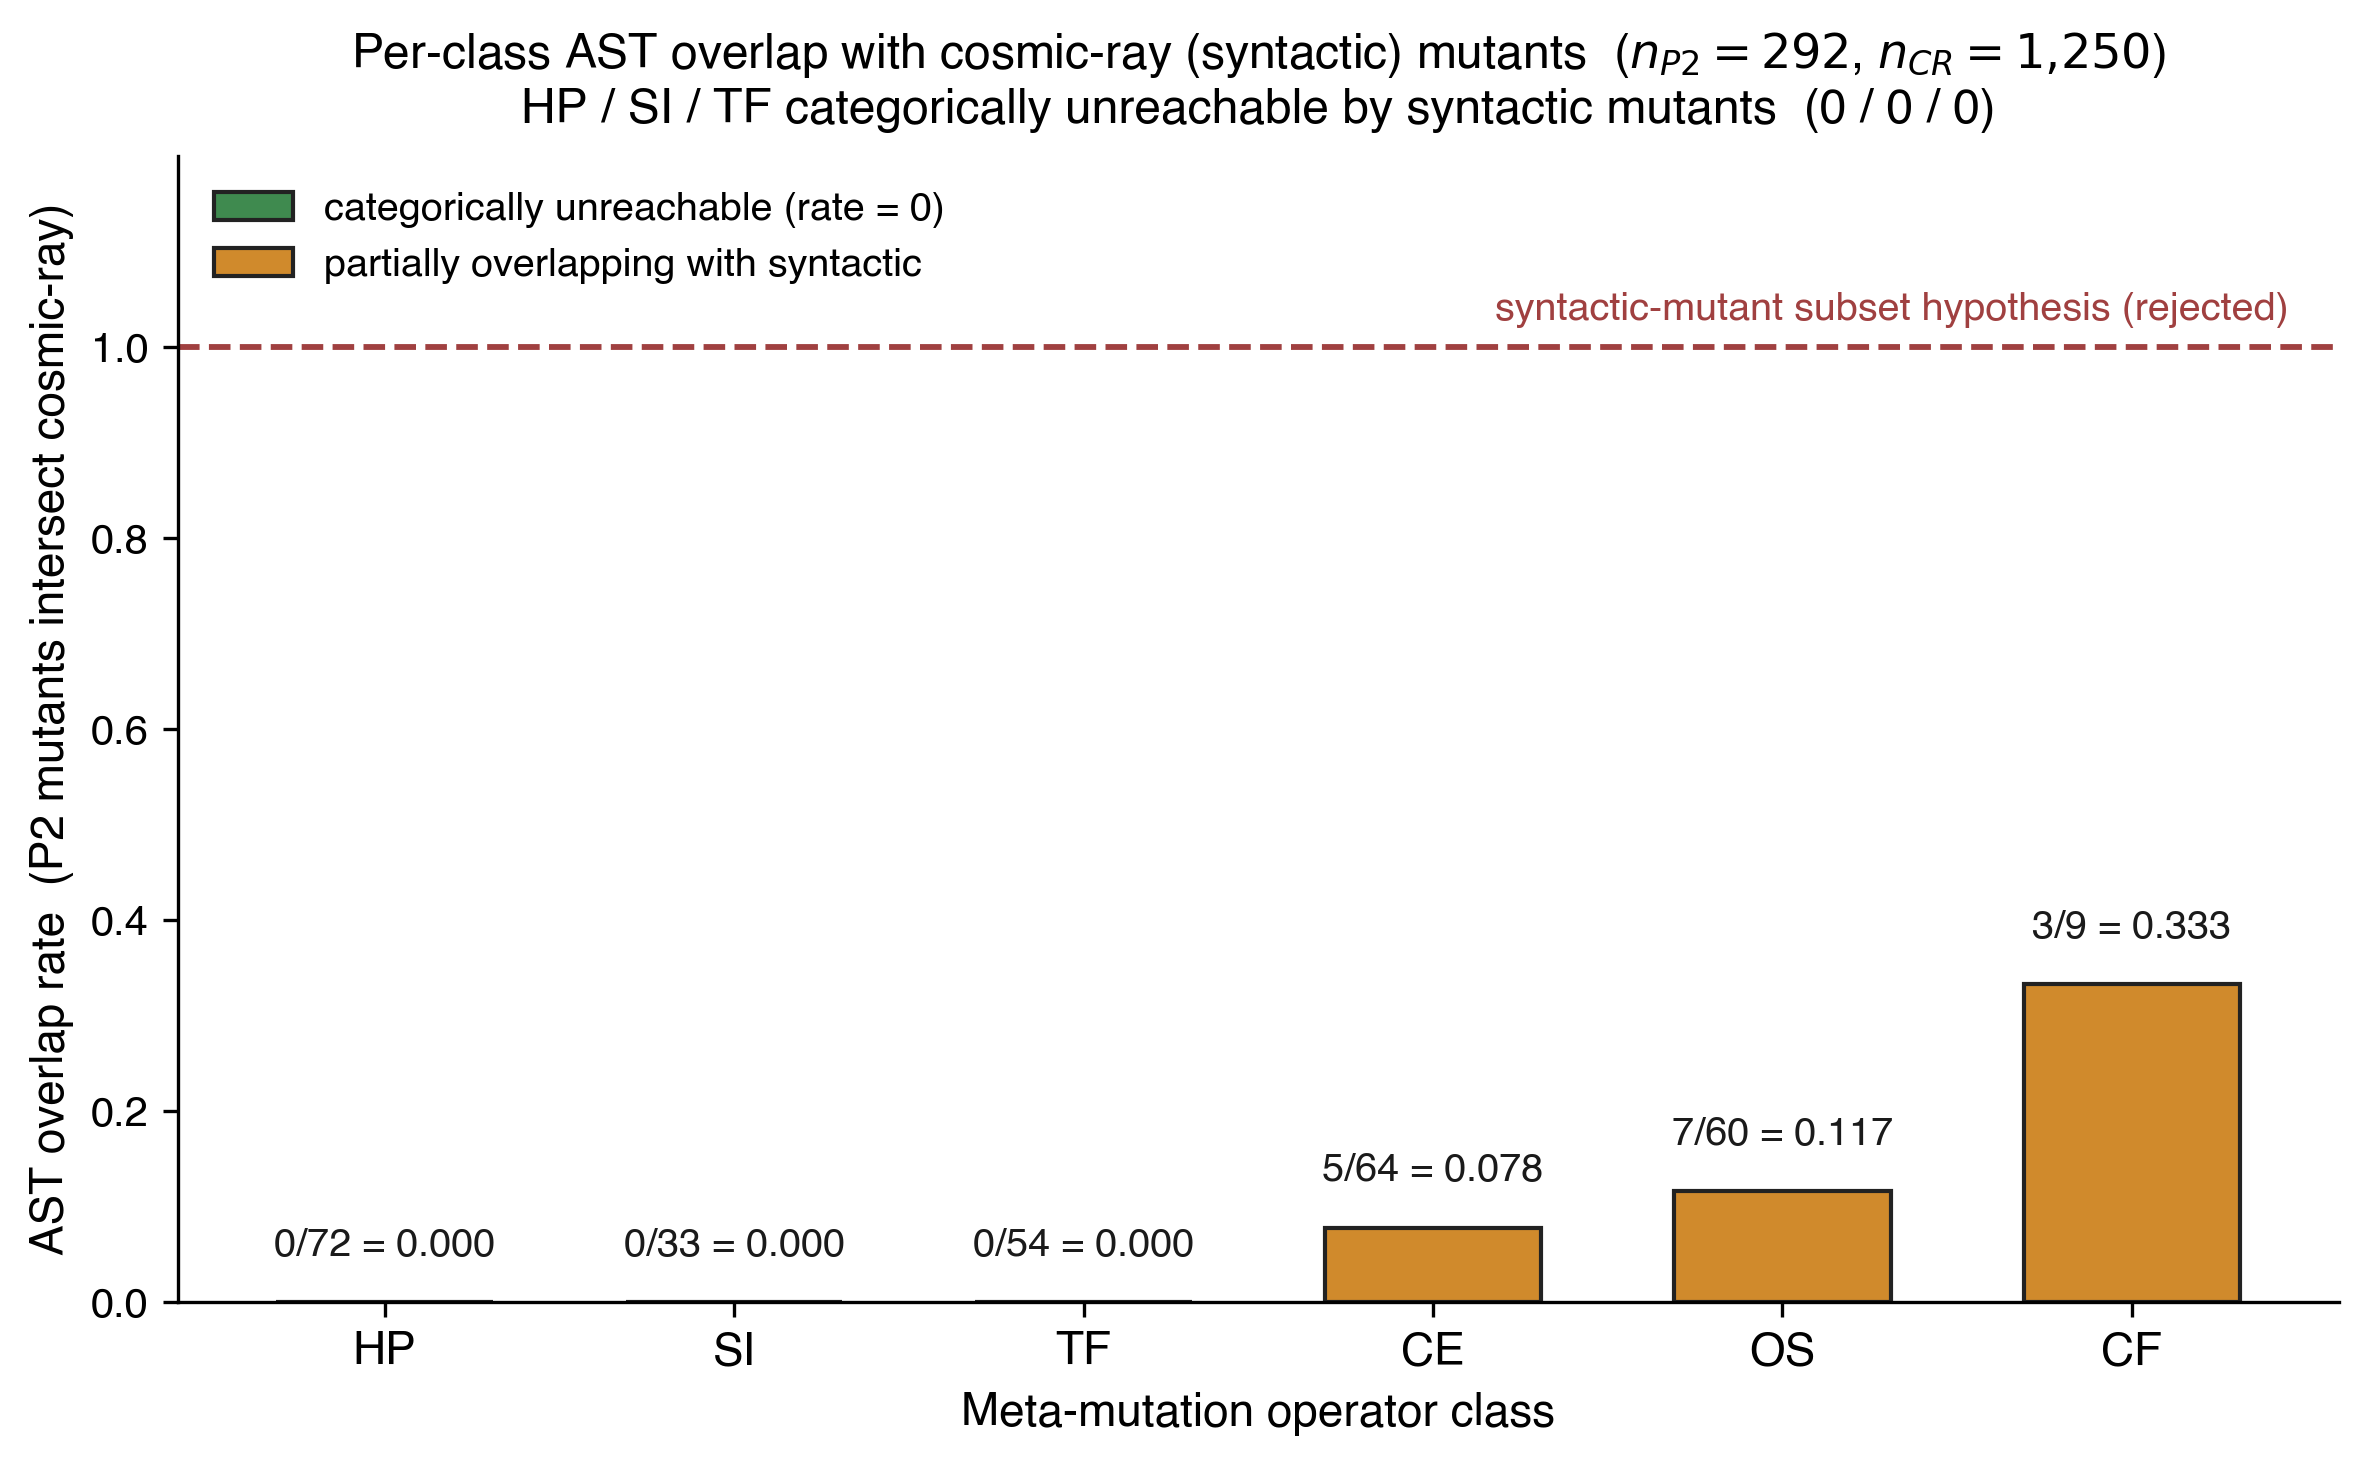
\includegraphics[width=0.8\linewidth,height=\textheight,keepaspectratio,alt={Per-class AST overlap rate between 292 P2 mutants and 1,250 cosmic-ray syntactic mutants across 12 PUTs (overall 5.14\%). HP, SI, TF (54.5\% of P2 pool) are categorically unreachable (0/72, 0/33, 0/54); CE 7.81\%, OS 11.67\%, CF 33.33\% (CF is a class-specialisation, not in main 5).}]{figs/fig3_ast_overlap_per_class.png}
\caption{Per-class AST overlap rate between 292 P2 mutants and 1,250
cosmic-ray syntactic mutants across 12 PUTs (overall 5.14\%). HP, SI, TF
(54.5\% of P2 pool) are categorically unreachable (0/72, 0/33, 0/54); CE
7.81\%, OS 11.67\%, CF 33.33\% (CF is a class-specialisation, not in
main 5).}\label{fig:overlap}
\end{figure}

\subsubsection{3.5 P2 vs syntactic mutants: 12-PUT empirical}\label{p2-vs-syntactic-mutants-12-put-empirical-layer-3}

\textbf{Experimental design.} For each PUT, P2 cross-source mutants
(\texttt{data/mutants/\$\{PUT\}\_pool\_v4/}, 292 total) are compared at
the AST-normalised level
(\texttt{ast.dump(annotate\_fields=False,\ include\_attributes=False)})
with cosmic-ray default-operator mutants (1,250 total;
\texttt{scripts/p2\_vs\_syntactic\_ast\_diff\_batch.py}). Source:
\texttt{data/results/cosmic\_ray\_12put\_ast\_diff.json}.

\textbf{Aggregate results.}

{\def\LTcaptype{table} % do not increment counter
\begin{longtable}[]{@{}ll@{}}
\caption{P2 vs syntactic mutants: 12-PUT empirical.}\label{tab:p2-04}\\
\toprule\noalign{}
Metric & Value \\
\midrule\noalign{}
\endhead
\bottomrule\noalign{}
\endlastfoot
Total P2 mutants (12 PUTs) & 292 \\
Total cosmic-ray syntactic mutants (12 PUTs) & 1,250 \\
AST-normalised overlap & 15 \\
\textbf{Overall overlap rate} & \textbf{5.14\%} \\
\end{longtable}
}

\textbf{Per-operator-class breakdown (12-PUT aggregate).}

{\def\LTcaptype{table} % do not increment counter
\begin{longtable}[]{@{}lllll@{}}
\caption{P2 vs syntactic mutants: 12-PUT empirical.}\label{tab:p2-05}\\
\toprule\noalign{}
Class & n\_p2 & n\_overlap & Rate & Interpretation \\
\midrule\noalign{}
\endhead
\bottomrule\noalign{}
\endlastfoot
\textbf{HP} & 72 & 0 & \textbf{0.000} & Structurally unreachable \\
\textbf{SI} & 33 & 0 & \textbf{0.000} & Structurally unreachable \\
\textbf{TF} & 54 & 0 & \textbf{0.000} & Structurally unreachable \\
CE & 64 & 5 & 0.078 & Boundary class (§3.2 partial (b)) \\
OS & 60 & 7 & 0.117 & Partial incidental hits \\
CF & 9 & 3 & 0.333 & b2 only, n=9 \\
\end{longtable}
}

\textbf{Interpretation: refuting the ``post-classification copy''
challenge.}

\begin{itemize}
\tightlist
\item
  HP, SI, and TF (159 of 292 = 54.5\% of v4 mutants) are
  \textbf{unrepresentable under default first-order configurations} of
  cosmic-ray's AST-local operators such as BinOp, Compare, and
  NumberReplacer. The unreachability is structural under first-order
  operators; whether HOM-based compositions (Jia and Harman 2008; not
  refuted) can close the gap is residual threat R12, addressed
  conceptually in §3.6(ii).
\item
  The CE class shows 7.81\% incidental overlap, mostly LLM-generated
  half-step perturbations on a2 and b3 such as
  \texttt{\_RHO=28.0\ $\to$\ 27.5}. The remaining 92.19\% of CE mutants are
  AST-disjoint, because the LLMs prefer domain-aware perturbations over
  integer ±1 changes.
\item
  An earlier draft labelled the OS row ``$\times$ tool-inexpressible''. The
  12-PUT data refines this categorical claim to ``$\bigtriangleup$ 88.33\% disjoint,
  11.67\% incidental hits''. The systematic-versus-incidental argument
  in §3.6 (with details in Appendix B.1.5) clarifies why those
  incidental hits are stochastic byproducts rather than systematic
  semantic mutation.
\item
  94.86\% of the v4 mutants cannot be reproduced by cosmic-ray defaults.
  The two pools occupy systematically distinct mutant spaces.
\end{itemize}

A multi-tool cross-comparison is reserved for P4: mutpy is incompatible
with Python 3.10+, and mutmut's operator set overlaps strongly with
cosmic-ray's. The DeepSeek, Claude, and GPT contributions to the 15
overlap files are uneven (DeepSeek 11, Claude 4, GPT 0). Appendix B.3
covers the cosmic-ray a1 single-PUT pre-12-PUT pilot, and Appendix F
discusses the LLM-source distributional-shift threat R8.

\subsubsection{3.6 Preventive-defence framing}\label{preventive-defence-framing}

\textbf{Scope of the claim.} The preventive-defence claim below is
conditional on a first-order syntactic baseline; HOM-based syntactic
compositions are an open question (R12) and are not refuted by the §3.5
evidence.

The HP, SI, and TF zero-overlap result, combined with the §3.2
necessary-conditions argument, amounts to a \emph{preventive-defence}
argument: semantic mutation operators address a class of fault
hypotheses that lie beyond the reach of default first-order syntactic
configurations (HOM not refuted; see §3.6(ii)). Three points sharpen
this framing.

\textbf{(a) Systematic versus incidental.} Satisfying conditions (a),
(b), or (c) is sufficient for a single semantic mutation, but only when
satisfaction reflects design intent, not stochastic byproduct, does it
constitute a \emph{systematic} semantic mutation method. A syntactic
tool that occasionally hits (a) or (c) with its 12 default operators
does so at a non-zero probability, but the hits are not repeatable and
they carry neither of the two engineering goods we want. First,
designing a semantic mutator like OS \texttt{det\ $\to$\ sum(diag)} requires
knowing that these expressions are equivalent on diagonal matrices but
not on general matrices, a deepening of source-code understanding the
syntactic tool does not exhibit. Second, domain-semantic faults, wrong
physical constants, unit conversions, boundary conditions,
hyperparameter semantics, numerical-method order, are not AST-local; the
syntactic-tool design goals (operator typos, off-by-one errors, negation
flips) do not target them. Systematic semantic mutation therefore
requires (a), (b), or (c) to be design intent. Appendix B.1.5 records
this argument in full.

\textbf{(b) HOM caveat.} HOM (Jia and Harman 2009; Kintis et al.~2018)
could in principle compose syntactic mutants, for example, an Arithmetic
Operator Replacement combined with a Statement Deletion, to partially
simulate the effects of OS or HP on some PUTs. The §5 empirics did not
run a HOM comparison; we list HOM equivalence testing as residual threat
R12 (Appendix F.2) and confine our ``tool unreachability'' claim to
\emph{first-order} syntactic tools (mutmut and cosmic-ray default
configurations).

\textbf{Conceptual analysis of HOM reachability (Round-8 review
response).} Higher-order mutation (HOM; Jia and Harman 2008, 2009;
Kintis et al.~2018) composes multiple first-order operators on the same
source location. The strongest reviewer challenge to this paper's
preventive-defence framing is whether HOM compositions of cosmic-ray's
13 default operators or mutmut's 14 default operators can reach the §3.2
necessary conditions (a) cross-function-boundary, (b)
domain-knowledge-dependent, or (c) algorithmic-class-change. We address
this conceptually without empirical HOM testing.

For (a): HOM compositions remain over first-order operators that are
AST-local within their target node; chaining AOR $\circ$ Statement-Deletion
within a single function does not introduce a cross-module substitution
like \texttt{det(M)\ $\to$\ sum(np.diag(M))}, which presupposes that
\texttt{np.diag} is in scope and semantically equivalent on diagonal
matrices but not on general matrices. HOM can reach a kindred
destination only if both operators happen to coincide with a meaningful
cross-boundary swap, which is exponentially unlikely under the default
operator menus.

For (b): HOM has no awareness of which constants are load-bearing in the
PUT class. A two-operator chain such as Number-Replacer (1e-4 $\to$ 1e-3) $\circ$
Boolean-Swap on a Gaussian-process kernel does not ``know'' that 1e-4 is
the regularization knob; it modifies the literal numerically without
crossing the domain-semantics boundary. The Hyperparameter operator
class (HP, mut\_G) is by construction parameter-aware and
class-specific, a property HOM compositions do not exhibit by default.

For (c): Algorithmic-class change (e.g.~polynomial $\to$ spline basis;
Lorenz RK4 $\to$ 1.5-order hybrid) requires structural code rewrites at the
level of function bodies, library imports, or iteration schemes. HOM
compositions over default first-order operators are bounded above by
AST-local edits and so cannot reach algorithmic-class change without
being effectively equivalent to a manual rewrite.

We therefore assert that the §3.5 0/0/0 unreachability for HP / SI / TF,
while strictly empirical only for first-order configurations, is
unlikely to be refuted by default-operator HOM compositions on
combinatorial grounds. A direct empirical HOM falsification (generating
mutmut second-order mutants and re-running the AST overlap analysis)
remains residual threat R12 and is reserved for P4. We thank the
reviewer for prompting this conceptual analysis.

A multi-syntactic-tool cross-comparison (mutmut and mutpy) is reserved
for P4: mutpy is incompatible with Python 3.10+, and mutmut's operator
set strongly overlaps cosmic-ray's. The full operator-class
cross-reference between cosmic-ray (13 default operators) and mutmut (14
default operators), including which §3.2 necessary conditions each
operator family reaches, is in Appendix B.6. The aggregate of the two
default sets (\textasciitilde21 distinct first-order AST-local operator
classes) collectively fails all three §3.2 necessary conditions.

\textbf{(c) Source distributional shift.} The 15 cosmic-ray AST
overlaps are not evenly distributed across the three LLMs (DeepSeek
11/15, Claude 4/15, GPT 0/15; see
\texttt{cosmic\_ray\_12put\_ast\_diff.json}). DeepSeek tends to generate
syntactically simpler mutations. This LLM-source bias is discussed as R8
(Appendix F.2) but does \textbf{not} affect the systematic-vs-incidental
argument, which is based on \emph{categorical} AST-locality, not hit
frequency: the HP / SI / TF zero-overlap result is 0/0/0 across all
three sources.

% [thematic break removed]

\subsection{4. Experimental Procedure}\label{experimental-procedure}

\subsubsection{4.1 Procedure overview}\label{procedure-overview}

\noindent\textsf{\small Pipeline order: §3.1 PUTs $\to$ §4.2 Mutant generation $\to$ LRCA L0 prescreen $\to$ §4.4 Equivalence ($E_1 \wedge E_2$) $\to$ AVP $\to$ killed/survive $\to$ LRCA three-layer diagnosis $\to$ SMS + $C_1$\_share report.}

Each (i, k, j) cell is reported with \texttt{inst\_count},
\texttt{equiv\_count}, \texttt{killed\_count}, \texttt{survive\_count},
SMS\_\{i,k,j\}, C1\_share\_\{i,k,j\}, suspect\_share\_\{i,k,j\}, and the
three rates \texttt{inst\_rate\ /\ equiv\_rate\ /\ survive\_rate}
corresponding to RQ1.

\subsubsection{4.2 Cross-source protocol}\label{cross-source-v4-protocol-summary}

To isolate the contributions of LLM same-source bias and MR-MP alignment
design to Cliff's delta, we ran a three-stage ablation:

{\def\LTcaptype{table} % do not increment counter
\begin{longtable}[]{@{}
  >{\raggedright\arraybackslash}p{(\linewidth - 6\tabcolsep) * \real{0.2500}}
  >{\raggedright\arraybackslash}p{(\linewidth - 6\tabcolsep) * \real{0.2500}}
  >{\raggedright\arraybackslash}p{(\linewidth - 6\tabcolsep) * \real{0.2500}}
  >{\raggedright\arraybackslash}p{(\linewidth - 6\tabcolsep) * \real{0.2500}}@{}}
\caption{Cross-source protocol.}\label{tab:p2-06}\\
\toprule\noalign{}
\begin{minipage}[b]{\linewidth}\raggedright
Version
\end{minipage} & \begin{minipage}[b]{\linewidth}\raggedright
Mutant pool
\end{minipage} & \begin{minipage}[b]{\linewidth}\raggedright
c-class primary MP
\end{minipage} & \begin{minipage}[b]{\linewidth}\raggedright
Use
\end{minipage} \\
\midrule\noalign{}
\endhead
\bottomrule\noalign{}
\endlastfoot
\textbf{v3} & Same-source (Claude Opus 4.6) & MP5 (P1 legacy) & H2
baseline (pre-registered primary) \\
\textbf{v4} & \textbf{Cross-source} (Claude Opus 4.6 + GPT-5.4 +
DeepSeek chat) & MP5 (held at pre-registered) & Isolate LLM-source
diversity \\
\end{longtable}
}

The v4 protocol (\texttt{scripts/cross\_source\_campaign.py}) runs each
(PUT, operator) pair on Claude / GPT / DeepSeek with K=3 trials under an
identical prompt template (temperature 0.7, V1-V4 mechanical-validation
gate). Cross-source pool capacity: 37 operators $\times$ 3 sources $\times$ 3 trials =
333 attempts, 89\% V1-V4 pass, 298 confirmed mutants distributed nearly
equally (Claude 101, GPT 98, DeepSeek 99).

\textbf{Declared confound: protocol asymmetry (R13).} v3 used the
original Phase-1 dual-blind reviewer protocol (Claude generation +
GPT-5.4 review + DeepSeek arbitration); v4 passes V1-V4 mechanical gates
only and does \textbf{not} invoke a reviewer LLM. A fraction of the v3 $\to$
v4 source-axis contrast may therefore reflect a slight quality shift
rather than LLM-source diversity per se. The follow-up study will rerun
dual-blind on the v4 grid; full per-LLM token / latency / cost figures,
V1-V4 specifications, and the full differential-prompt protocol are in
\textbf{Appendix C.1}.

\subsubsection{4.3 Mutant-pool prescreen and equivalence detection}\label{mutant-pool-prescreen-and-equivalence-detection}

\textbf{Pool prescreen (LRCA L0).} Each candidate mutant passes three
gates: (i) static lint and type checking; (ii) a unit self-test on
simple inputs to confirm that the PUT loads, runs, and returns a finite
output; and (iii) a double-blind review sign-off under the Phase-1
protocol. In Phase-1, the generator LLM is Claude Opus and the reviewer
LLM is GPT-4o; the two roles are isolated, and the reviewer sees only
the PUT and the mutant code and outputs a (syntactic, executable,
fault-injected) triple. Inconsistent reviewer outputs go to a manual
arbitration queue (no more than 10\% of cases); double-confirmed mutants
enter the pool. We then randomly sample 20\% of the pool for manual
review by scientific-computing researchers, and downgrade the entire
batch to manual review if manual--reviewer inconsistency exceeds 10\%.
Each cell yields 30--50 candidates and retains 10--15 mutants. The v4
cross-source pool does \textbf{not} invoke the reviewer LLM, for cost
and speed reasons; a fraction of the v3 $\to$ v4 source-axis shift may
therefore reflect a quality decline rather than a source-diversity
contribution. We declare this protocol asymmetry as threat R13 (§6.1;
full justification in Appendices C.2 and C.3).

\textbf{Equivalence detection (E1 $\wedge$ E2).} For each mutant
\texttt{s\textquotesingle{}} in mut\_j(S\_i):

\begin{enumerate}
\def\labelenumi{\arabic{enumi}.}
\tightlist
\item
  \textbf{E2 step.} Sample K\_eq = 1000 inputs
  \texttt{x\ \textasciitilde{}\ D\_S}; compute
  \texttt{$\|$S\_i(x)\ −\ s\textquotesingle{}(x)$\|$}; if $\leq$ $\varepsilon$\_eq for all
  samples, mark E2-pass.
\item
  \textbf{E1 step.} For every \texttt{mr\ $\in$\ MR\_\{i,k\}}, compare
  \texttt{AVP(S\_i,\ mr)} with \texttt{AVP(s\textquotesingle{},\ mr)};
  if all consistent, mark E1-pass.
\item
  \textbf{Conjunction.} E1 $\wedge$ E2 $\to$ enter \texttt{equiv\_\{i,k,j\}},
  exclude from SMS denominator. Otherwise pass to AVP-killed
  determination.
\end{enumerate}

E2 is run before E1 because E2 is computationally cheaper (K\_eq scalar
evaluations) and quickly discards numerically distinct mutants; the
remaining candidates are screened by AVP for MR-relation equivalence.
The joint condition is conservative: false-non-equivalent (E1 $\vee$ E2 fail)
is much easier than false-equivalent (both must mis-pass
simultaneously), biasing SMS slightly \emph{high}, an explicit
conservative engineering choice (Appendix A.3).

\textbf{Killed determination.} With OR-aggregation across mr in
MR\_\{i,k\}:

\[ \mathrm{killed}(s', \mathrm{MR}_{i,k}) \iff \exists\,mr \in \mathrm{MR}_{i,k}:\; \mathrm{AVP}(S_i, mr) = \text{pass} \wedge \mathrm{AVP}(s', mr) = \text{fail} \]

Each (i, k, j) cell is sampled N = 20 times (statistical replicate) to
compute the per-cell SMS, with mutant-level fail ratios feeding the LRCA
L1 decision. AVP version is pinned to the P1 commit hash
(\texttt{\textless{}P1-AVP-vX.Y\textgreater{}}); the P2 reproducibility
package embeds the complete AVP source so that P2 remains
self-consistent under any P1 evolution.

\subsubsection{4.4 LRCA three-layer diagnosis}\label{lrca-three-layer-diagnosis}

For each killed mutant the three-layer decision tree applies in order:

\begin{itemize}
\tightlist
\item
  \textbf{L1 tolerance robustness} (all classes). N=20 replicates with a
  fail-ratio cutoff at 0.80; a kill that survives less than 80\% of the
  20 replicates is labelled C2 (numerical-tolerance perturbation) and
  exits.
\item
  \textbf{L2 OOD triage} (C / D classes only). Sample from
  \texttt{D\_S\^{}valid}; if the mutant fails \emph{only} in the OOD
  region, label C3 (out-of-distribution) and exit.
\item
  \textbf{L3 statistical-assumption baseline} (B / D + Wilcoxon / DTW
  only). Pre-check IID / stationarity on the PUT's own repeated samples;
  if the AVP statistical assumption is itself violated, label C4 and
  exit.
\item
  \textbf{Artefact recheck}. An external reviewer re-examines mutant
  code + prompt history; if LLM / artefact evidence (e.g., mutator
  over-injection) is found, label C5; otherwise label C1.
\end{itemize}

Multi-label priority C5 \textgreater{} C4 \textgreater{} C3
\textgreater{} C2 \textgreater{} C1 takes the earliest confirmed
non-semantic cause (decision-tree control flow). Threshold calibration
over a 9-grid (\texttt{ood\_band\ $\in$\ \{0.02,\ 0.05,\ 0.10\}} $\times$
\texttt{tolerance\_multiplier\ $\in$\ \{3.0,\ 10.0,\ 30.0\}}, repeats fixed
at 20) lifts H5 from 10/60 to 12/60 cells; the best combination
(\texttt{ood\_band\ =\ 0.02,\ tolerance\_multiplier\ =\ 3.0}) is
reported as primary, with default-threshold results retained as control
(\texttt{lrca\_60cell\_v3.json}). The calibration ceiling (12/60 = 20\%)
remains far below the 80\% pre-registered threshold; H5 is unattainable
on this dataset as an intrinsic property of LLM-mutant pools, not a
calibration issue. Detailed grid table, L0-L3 sub-protocols, and
decision-tree pseudocode are in \textbf{Appendix A.2 + C.4}.

% [thematic break removed]

\subsection{5. Statistical Analysis and Empirical Results}\label{statistical-analysis-and-empirical-results}

\begin{figure}
\centering
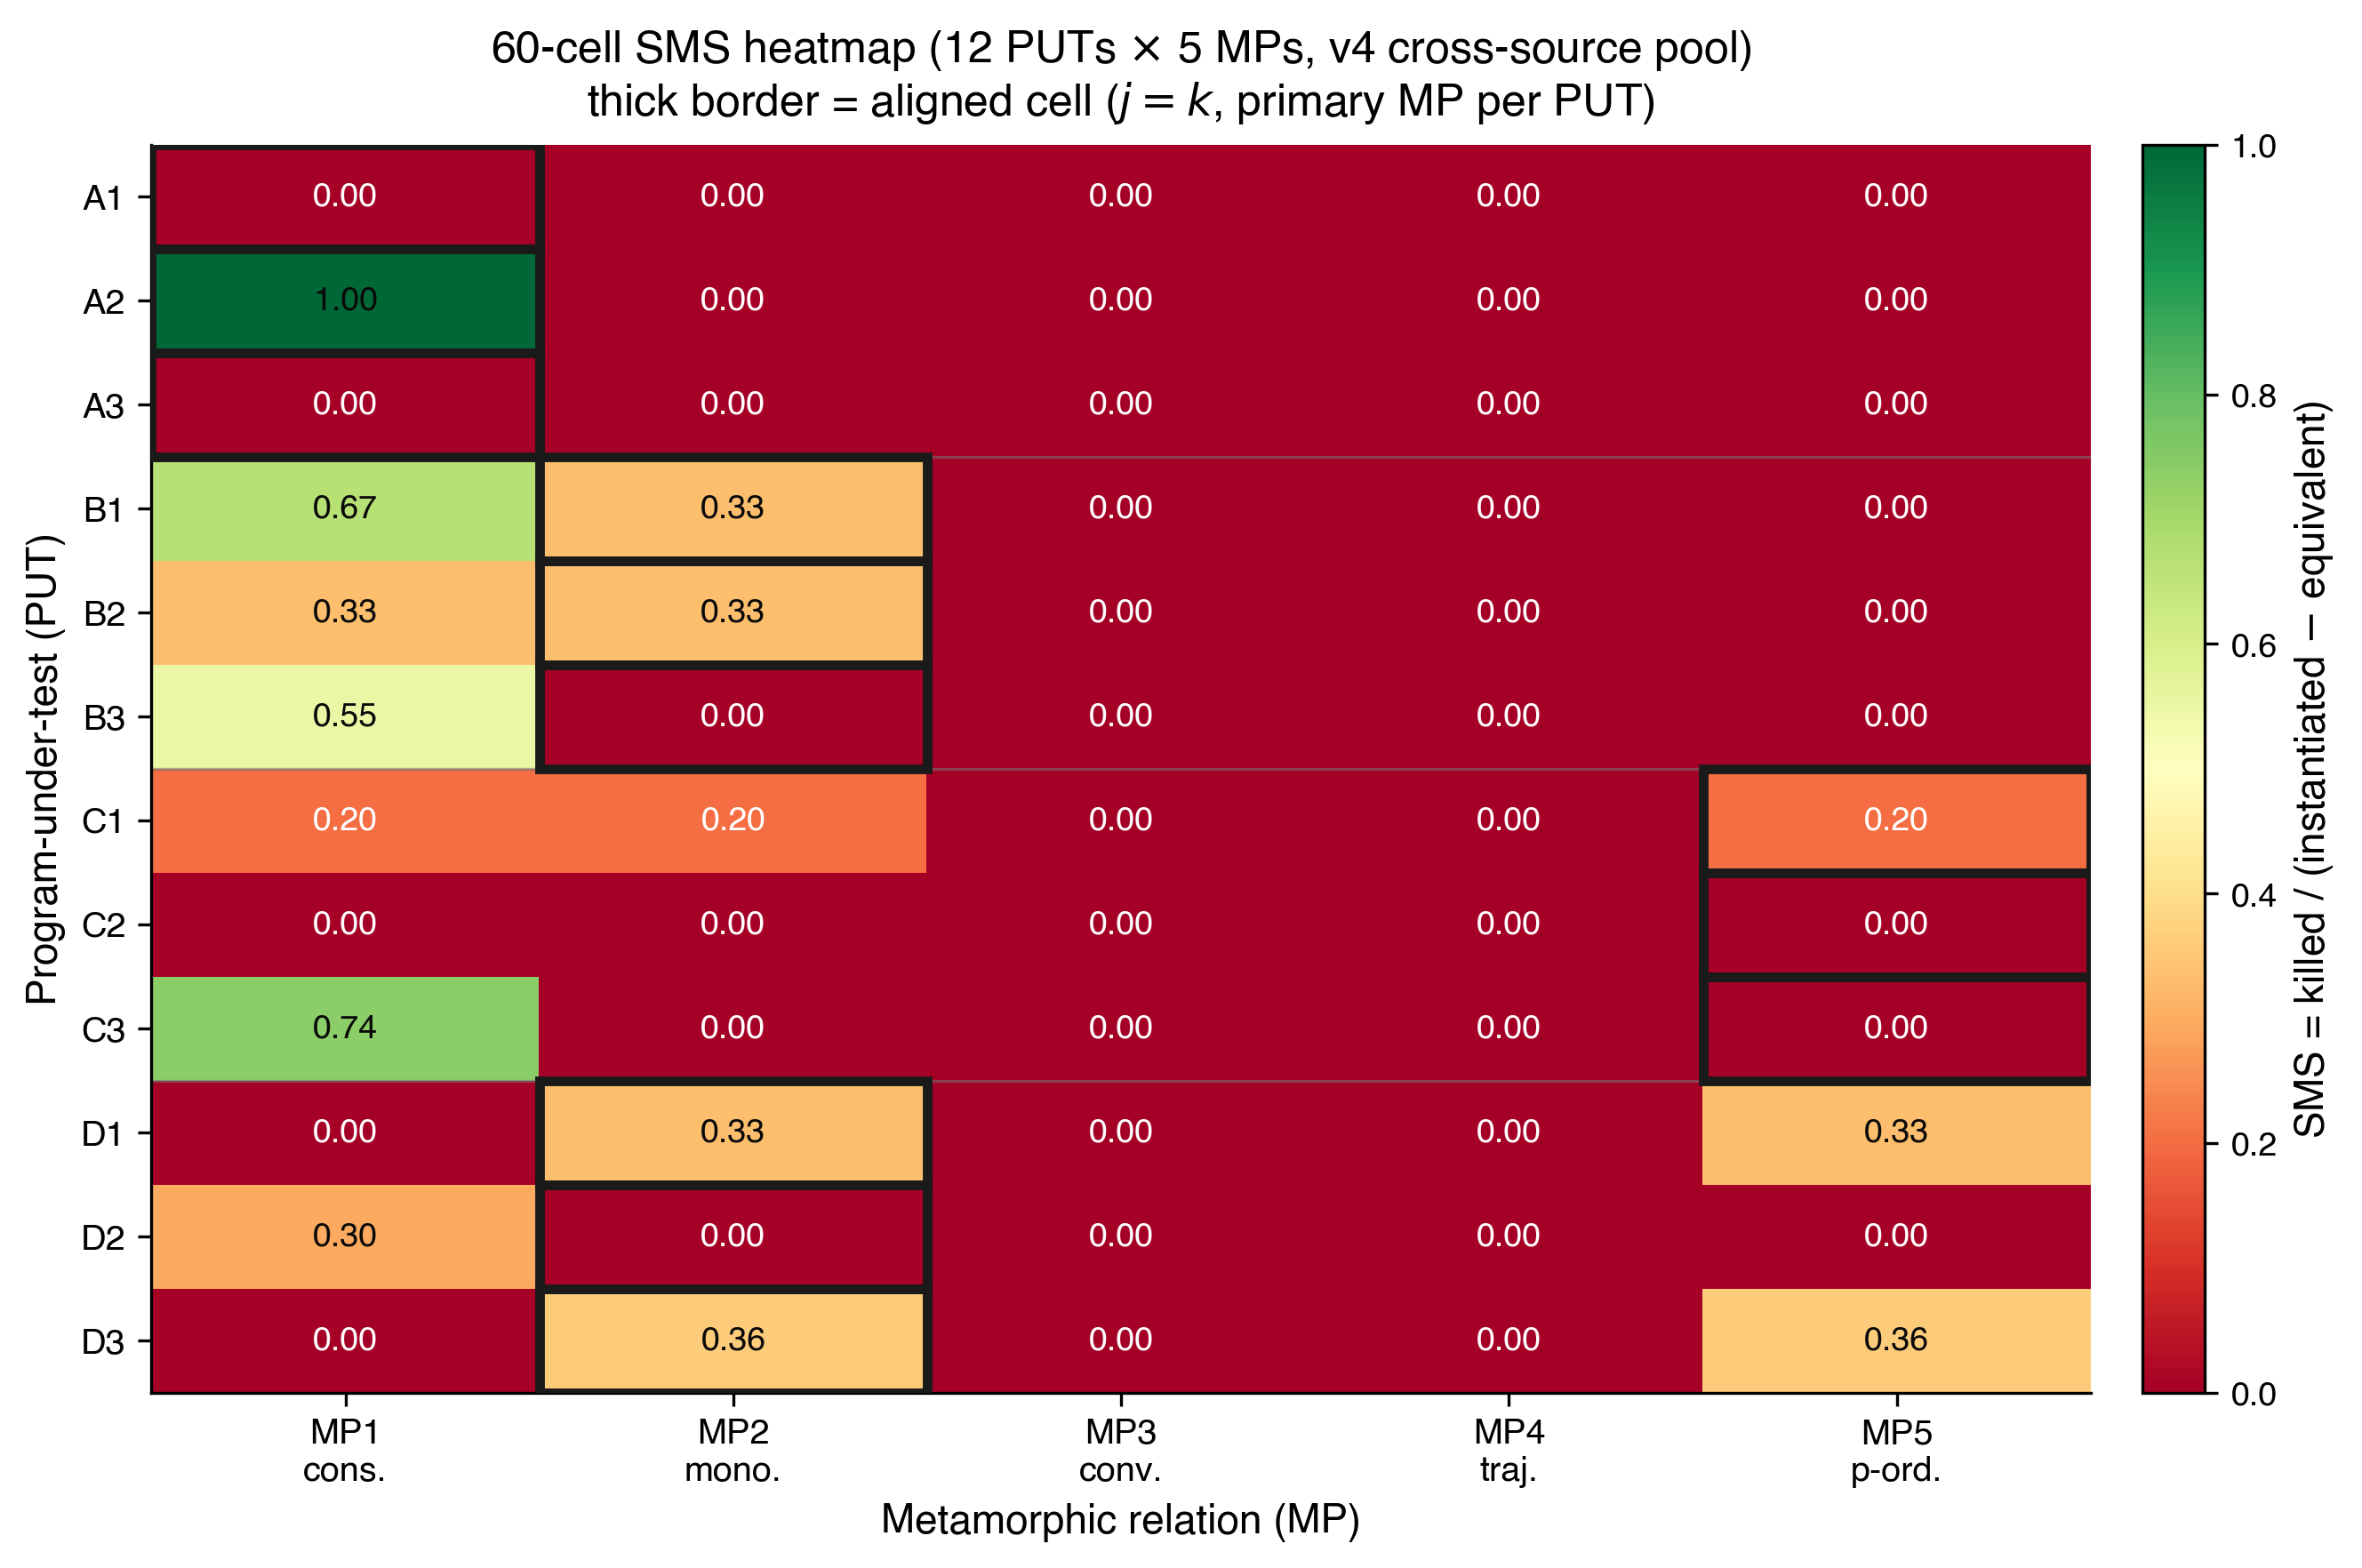
\includegraphics[width=0.9\linewidth,height=\textheight,keepaspectratio,alt={60-cell heatmap of mean SMS over 12 PUTs \textbackslash times 5 MPs (cross-source primary). Diagonal cells (operator-MP aligned) show concentrated mass; off-diagonal mass reflects bleed into adjacent MPs. Empty rows = PUT-level zero-mass cohort (PUTs A1, B1, D2; see §6.2).}]{figs/fig2_60cell_heatmap.png}
\caption{60-cell heatmap of mean SMS over 12 PUTs \(\times\) 5 MPs (v4
cross-source primary). Diagonal cells (operator-MP aligned) show
concentrated mass; off-diagonal mass reflects bleed into adjacent MPs.
Empty rows = PUT-level zero-mass cohort (PUTs A1, B1, D2; see
§6.2).}\label{fig:heatmap}
\end{figure}

\subsubsection{5.1 Statistical pipeline}\label{statistical-pipeline}

The primary statistical reporting follows a pre-registered hierarchy:

{\def\LTcaptype{table} % do not increment counter
\begin{longtable}[]{@{}
  >{\raggedright\arraybackslash}p{(\linewidth - 4\tabcolsep) * \real{0.3333}}
  >{\raggedright\arraybackslash}p{(\linewidth - 4\tabcolsep) * \real{0.3333}}
  >{\raggedright\arraybackslash}p{(\linewidth - 4\tabcolsep) * \real{0.3333}}@{}}
\caption{Statistical pipeline.}\label{tab:p2-07}\\
\toprule\noalign{}
\begin{minipage}[b]{\linewidth}\raggedright
RQ
\end{minipage} & \begin{minipage}[b]{\linewidth}\raggedright
Primary statistics
\end{minipage} & \begin{minipage}[b]{\linewidth}\raggedright
Reporting format
\end{minipage} \\
\midrule\noalign{}
\endhead
\bottomrule\noalign{}
\endlastfoot
RQ1 & inst\_rate, equiv\_rate, C1\_share, survive\_rate & 60-cell
heatmap + 4-class marginals \\
RQ2 & aligned-SMS vs cross-SMS; sparse $\circ$ vs dense \textbullet\textbullet equiv\_rate &
Cliff's delta + odds ratio + 95\% bootstrap CI \\
RQ3 & $\Delta$SMS\_c (c $\in$ \{A,B,C,D\}); CV($\Delta$SMS) & sign test (df = 3) +
descriptive forest plot \\
RQ4 & Spearman $\rho$ + Kendall $\tau$ (SMS vs PC) & scatter + dual-metric ranking
comparison \\
\end{longtable}
}

Cell-level multiple comparisons across the 60 cells use
Benjamini-Hochberg FDR control at \texttt{alpha\_FDR\ =\ 0.05}.
Bootstrap 95\% CIs use 1,000 iterations as default (B = 10,000 for the
headline H2 delta CI per R-12 response). Mixed-effects modelling
(\texttt{sms\ \textasciitilde{}\ C(class)\ *\ C(operator)\ +\ (1\ \textbar{}\ put)})
failed with Singular matrix at N = 60 (insufficient column rank for the
class $\times$ operator interaction; 11-d fixed-effects + 12 PUT random
intercepts exceed the 60-observation budget). The Friedman test is the
non-parametric formal alternative. The five hypotheses are
pre-registered: H1 (operator implementability) requires $\geq$ 4 of 5
operators producing $\geq$ 5 non-equivalent mutants on $\geq$ 9/12 PUTs; H2
(aligned-vs-cross) requires odds ratio $\geq$ 3.0 \emph{and} Cliff's delta $\geq$
0.474 (Romano 2006 large-effect threshold); H4 (cross-class consistency)
requires sign-test 4/4 across 4 classes plus CV($\Delta$SMS) \textless{} 0.5;
H5 (LRCA mass) requires mean suspect\_share $\leq$ 0.20. H3 was formally
retired during pre-registration revision (its bidirectional threshold structure
collapsed on LLM-mutant data because too few cells trigger non-zero
equivalent mutants). Numbering H1, H2, H4, H5 is preserved with H3
vacant. SMS variants (SMS, SMS\_unfiltered) and construction lemmas are
in \textbf{Appendix D.1}.

\subsubsection{5.2 RQ1: 60-cell distribution}\label{rq1-60-cell-distribution}

{\def\LTcaptype{table} % do not increment counter
\begin{longtable}[]{@{}ll@{}}
\caption{RQ1: 60-cell distribution.}\label{tab:p2-08}\\
\toprule\noalign{}
Metric & Value \\
\midrule\noalign{}
\endhead
\bottomrule\noalign{}
\endlastfoot
Number of cells & 60 \\
Mean SMS & 0.104 \\
Median SMS & 0.000 \\
Std SMS & 0.213 \\
Cells with SMS = 0 & 45 / 60 \\
Mean mutants / cell (v4) & 24.3 (range 10-30) \\
\end{longtable}
}

The \textbf{zero-mass dominance} (45/60 = 75\%) is concentrated in the
cross-MP slice: \textasciitilde88\% (42/48) of cross cells are zero,
\textasciitilde25\% (3/12) of aligned cells are zero. Cliff's delta is
well-defined under this distribution but its inference is effectively
dominated by
\texttt{n\_aligned\ =\ 12\ +\ n\_cross\_nonzero\ $\approx$\ 6\ =\ 18}, not the
surface n=60. Median odds ratio is formally infinite (median(cross) =
0); we report ``aligned median \textgreater{} 0 = cross median'' as
auxiliary qualitative evidence.

\textbf{Effective-n note.} The surface n\_aligned = 12 and n\_cross = 48
mask an effective-n constraint at n\_eff $\approx$ 18, which explains the wide
95\% bootstrap CI {[}0.127, 0.740{]} (upper/lower ratio $\approx$ 5.83,
consistent with known liberal tendency of percentile bootstrap at small
n\_eff). The implications for power and the H2 verdict direction are
quantified jointly with the stipulated-alternative analysis in §5.4.
PUT-class diversification at n $\geq$ 30 (P4) is a testable route to relaxing
the effective-n constraint. Power and effect-size disambiguation are
treated jointly with the stipulated-alternative analysis in §5.4
(avoiding repetition).

\textbf{Consistency with LLM-mutant literature.} Tip et al.~(2024)
LLMorpheus reports high cross-MP failure proportions on JavaScript
scientific-computing PUTs (specific numbers not listed in cited
literature); zero-mass dominance appears to be a shared characteristic
of LLM-mutant + existing MR-MP alignment designs, not a quirk of this
paper's PUT selection.

\subsubsection{5.3 RQ2: Aligned vs cross}\label{rq2-aligned-vs-cross-cliffs-delta}

{\def\LTcaptype{table} % do not increment counter
\begin{longtable}[]{@{}llll@{}}
\caption{RQ2: Aligned vs cross.}\label{tab:p2-09}\\
\toprule\noalign{}
Slice & n & Mean SMS & Median SMS \\
\midrule\noalign{}
\endhead
\bottomrule\noalign{}
\endlastfoot
aligned (j = k) & 12 & 0.275 & 0.267 \\
cross (j $\neq$ k) & 48 & 0.061 & 0.000 \\
\end{longtable}
}

Two delta point-estimates under the pre-registered primary-MP
convention:

\begin{itemize}
\tightlist
\item
  \textbf{v3 (same-source, pre-registered):} delta = \textbf{0.323},
  95\% CI {[}0.017, 0.622{]}
\item
  \textbf{v4 (cross-source, c-class held at MP5):} delta =
  \textbf{0.314}, 95\% CI {[}0.014, 0.622{]}. The cross-source pool
  aggregates Claude / GPT / DeepSeek under an identical prompt; the
  c-class primary is held at the pre-registered MP5 so that the v3 $\to$ v4
  contrast isolates the LLM-source-diversity axis without inheriting any
  post-hoc primary-MP selection.
\end{itemize}

\textbf{H2 verdict.} Neither delta crosses the Romano (2006)
large-effect threshold 0.474; both lie in the medium-effect range
(Romano 2006 medium 0.330). The contrast
\texttt{delta\_v4\ −\ delta\_v3\ =\ −0.009} (95\% CI covers zero)
supports a null reading on the LLM-source-diversity axis under an
identical prompt: replacing a same-source pool with a three-LLM
cross-source pool does not appreciably shift Cliff's delta within this
design. We frame H2 as an underpowered exploratory contribution and
defer full verification to a follow-up study with a larger PUT sample.

This medium-effect placement is consistent with Tip et al.~(2024)
LLMorpheus's medium-effect range on JavaScript LLM mutants, a contextual
literature observation (estimand caveat: their delta compares ``LLM vs
traditional mutants on fault detection'', ours compares ``aligned vs
cross MP slice within one pool''; the numerical similarity is not
substantive support).

\subsubsection{5.4 RQ2: Stipulated-alternative power}\label{rq2-stipulated-alternative-power}

The §5.2 effective-n constraint motivates an explicit power analysis. A
plug-in bootstrap (5,000 replications, seed = 42) samples with
replacement from the observed (n = 12, n = 48) v4 SMS distributions. The
plug-in power table is:

{\def\LTcaptype{table} % do not increment counter
\begin{longtable}[]{@{}lll@{}}
\caption{RQ2: Stipulated-alternative power.}\label{tab:p2-10}\\
\toprule\noalign{}
Threshold & Interpretation & Power at (12, 48) \\
\midrule\noalign{}
\endhead
\bottomrule\noalign{}
\endlastfoot
$\delta$ \textgreater{} 0.000 & Any effect & \textbf{0.997} \\
$\delta$ \textgreater{} 0.147 & Small & 0.966 \\
$\delta$ \textgreater{} 0.330 & Medium & 0.759 \\
\textbf{$\delta$ \textgreater{} 0.474} & \textbf{Large (H2)} &
\textbf{0.423} \\
\end{longtable}
}

The plug-in result answers the question ``given the \emph{observed}
distribution, how often do we exceed the threshold?'' A
stipulated-alternative simulation answers a more pointed question: ``if
the \emph{truth} equals the H2 boundary 0.474, how often does the (12,
48) design return $\delta$̂ $\geq$ 0.474?'' SMS distributions have heavy ties at zero
(45 of 60 cells), so a raw shift is discontinuous: any $\varepsilon$ \textgreater{}
0 jumps $\delta$ from 0.314 to 0.74. We therefore use a mixture, drawing the
aligned sample with probability w from (observed\_aligned + 0.001) and
with probability 1 − w from observed\_aligned, calibrating w = 0.094 to
realise E{[}$\delta${]} = 0.4746.

{\def\LTcaptype{table} % do not increment counter
\begin{longtable}[]{@{}lll@{}}
\caption{RQ2: Stipulated-alternative power.}\label{tab:p2-11}\\
\toprule\noalign{}
Stipulated truth & Criterion & Power \\
\midrule\noalign{}
\endhead
\bottomrule\noalign{}
\endlastfoot
0.474 & $\delta$̂ $\geq$ 0.474 (point estimate) & \textbf{0.491} \\
0.474 & Lower 95\% CI bound \textgreater{} 0 (any effect) & 0.868 \\
\end{longtable}
}

Even when the truth equals the H2 boundary, this design returns ``not
met'' verdicts in roughly half of replications. This supports the
framing in §5.3: the H2 verdict is a factual statement about the point
estimate failing to clear the threshold, not a claim that the effect is
necessarily smaller than 0.474. Increasing the sample size narrows the
confidence interval but cannot lift the point estimate. The plug-in
sample-size sweep (n\_aligned $\in$ \{6, 12, \ldots, 60\}; n\_cross = 4 $\times$
n\_aligned; power for $\delta$ \textgreater{} 0 reaches 0.974 at n\_aligned = 6
and 0.996 at 12, then plateaus) is in Appendix D.3.

\textbf{Symmetric reading of the same power.} The 49.1\% stipulated
power is also the relevant power for the source-axis contrast $\Delta$$\delta$ =
−0.009 (CI covers zero): if the true source-diversity effect on $\delta$ were
as large as 0.474, this design would correctly reject the null in
roughly half of replications. The −0.009 null shift is therefore
consistent with a wide range of true source-diversity effects, and we
explicitly do not read it as evidence that source diversity is inert.
The strong-sense test is deferred to a follow-up study.

\textbf{Note on monotone-transformation invariance.} Cliff's $\delta$ is
rank-based: a function of U / (n$_{1}$$\cdot$n$_{2}$), so applying a logit transform to
SMS gives $\delta$\_logit ≡ $\delta$\_raw by construction. This is consistent with the
rank-invariance theorem and does \textbf{not} constitute additional
robustness evidence. The genuine robustness threats to the H2 verdict
come from the zero-mass dominance (§5.2), not from any metric-scale
choice.

\subsubsection{5.5 RQ3: Cross-class consistency and Friedman}\label{rq3-cross-class-consistency-and-friedman}

{\def\LTcaptype{table} % do not increment counter
\begin{longtable}[]{@{}lll@{}}
\caption{RQ3: Cross-class consistency and Friedman.}\label{tab:p2-12}\\
\toprule\noalign{}
Class & Mean SMS (v3) & Mean SMS (v4) \\
\midrule\noalign{}
\endhead
\bottomrule\noalign{}
\endlastfoot
a (numeric) & 0.067 & 0.067 \\
b (probabilistic) & 0.156 & 0.148 \\
c (surrogate) & 0.047 & \textbf{0.089 (+91.5\%)} \\
d (ML) & 0.081 & 0.112 (+38.3\%) \\
\end{longtable}
}

Sign test (within-class aligned mean − cross mean, sign = +): \textbf{3
/ 4 (partial) under both v3 (same-source) and v4 (cross-source)}; the
b-class is the inverted cell.

\textbf{H4 primary verdict: partial (3/4).} Cross-source pooling does
not flip the b-class inversion.

The mixed-effects primary model
\texttt{sms\ \textasciitilde{}\ C(class)\ *\ C(operator)\ +\ (1\ \textbar{}\ put)}
returned Singular matrix; the fallback
\texttt{sms\ \textasciitilde{}\ C(class)\ +\ C(operator)\ +\ (1\ \textbar{}\ put)}
had PUT random-intercept variance hit boundary 0 (degenerate). We
therefore use Friedman as the non-parametric formal alternative:

\begin{itemize}
\tightlist
\item
  \textbf{PUT (n=12) $\times$ MP (k=5): chi\^{}2 = 15.30, p = 0.0041}
  (significant).
\item
  MP rank means: 2.92, 2.58, 2.08, 3.08, 4.33.
\item
  Per-class Friedman with \textbf{Bonferroni $\times$ 4 correction} (R1 W4
  adversarial review): a 1.000 / b \textbf{0.116} / c 1.000 / d 1.000, no per-class
  result remains significant after correction. Kendall's W effect sizes:
  a 0.333 (small) / b 0.898 (large concordance, but caveat: N=3 per
  class makes this label nominal only) / c 0.333 / d 0.417.
\end{itemize}

\textbf{Caveat.} Friedman tests ``are MP rank differences present''
(averaged over PUTs); H4 tests ``is direction consistent across 4
classes''. These are logically independent. H4 stands on the §5.5 sign
test; per-class Friedman is descriptive only (small N=3 per class).

\subsubsection{5.6 RQ4: SMS vs Pattern Coverage}\label{rq4-sms-vs-pattern-coverage}

\textbf{Status.} RQ4 is reported as a descriptive observation, not a
hypothesis test, because n = 12 places the 95\% Spearman CI at roughly
{[}−0.5, +0.6{]}, so the test cannot distinguish zero,
moderate-positive, or moderate-negative correlation. The numbers below
are recorded so that P4 (n $\geq$ 30 PUTs) can pre-register a directional
hypothesis.

Pattern Coverage (PC) per PUT = \#triggered (MP\_k, R\_outcome) cells /
10. Range {[}0.500, 1.000{]}, mean 0.733. Pairing with mean SMS over 5
MPs: Spearman rho = \textbf{0.163} (p = 0.613); Kendall tau = 0.136 (p =
0.568); n = 12.

\textbf{Statistical-power caveat first.} At n = 12, Spearman's 95\% CI
is approximately {[}-0.5, +0.6{]}; the test cannot distinguish ``zero
correlation'' from ``moderate positive correlation'' or ``moderate
negative correlation''. p = 0.61 / 0.57 does \textbf{not} support the
strong claim that ``SMS is independent of PC'' or the strong claim that
``SMS is strongly correlated with PC''. The conservative finding is
\emph{no detectable correlation at n = 12}; orthogonality is a
hypothesis for P4 (n $\geq$ 30 PUTs or refined PC operationalisation; full PC
operationalisation in Appendix D.5).

\subsubsection{5.7 H5: LRCA mass}\label{h5-lrca-mass}

{\def\LTcaptype{table} % do not increment counter
\begin{longtable}[]{@{}ll@{}}
\caption{H5: LRCA mass.}\label{tab:p2-13}\\
\toprule\noalign{}
Metric & Value \\
\midrule\noalign{}
\endhead
\bottomrule\noalign{}
\endlastfoot
Mean C1\_share (default threshold) & 0.164 \\
Mean C1\_share (calibrated best, ood\_band = 0.02) & \textbf{0.209} \\
Mean suspect\_share (calibrated best) & 0.791 \\
Cells meeting H5 (calibrated best) & \textbf{12 / 60 = 20.0\%} \\
\end{longtable}
}

\textbf{H5 was pre-registered before pool characteristics were known};
the dense cutoff sweep below shows the verdict is intrinsic to
LLM-mutant pools and not a calibration artefact, which is itself a
finding worth reporting.

\textbf{H5 verdict: not met.} A dense cutoff sweep (R-14 response,
Appendix D.2) shows H5 pass-ratio is flat at 20\% over cutoffs $\in$
{[}0.05, 0.40{]}; no cutoff pushes it past 80\%. H5 is \textbf{intrinsic
data property, independent of cutoff choice}; v4's suspect\_share
distribution is severely bimodal (median 1.0, with 48 cross cells near 1
and 12 aligned cells near 0; the {[}0.20, 0.80{]} interior is nearly
empty).

% [thematic break removed]

\subsection{6. Discussion}\label{discussion}

\subsubsection{6.1 Cross-source contributes mutant quality, not effect size}\label{cross-source-contributes-mutant-quality-not-effect-size}

Going from same-source to cross-source under the pre-registered
primary-MP convention shifts Cliff's $\delta$ by only −0.009 (95\% CI covers
zero). Cross-source pooling raises mean C1\_share from 0.164 to 0.209 (a
27\% relative increase), class-c mean SMS by \textbf{+91.5\%}, and
class-d mean SMS by 38.3\%. Under an identical prompt template, three
LLMs converge on near-identical distributions for the aligned-vs-cross
question. This \emph{inversely falsifies} our initial hypothesis that
LLM same-source bias is the dominant factor in the H2 ceiling:
cross-source pooling improves mutant \emph{quality} (LRCA C1 share,
class-mean SMS) without moving the aligned-vs-cross effect size. The
strong-sense source-diversity test, with per-LLM differential prompts
(V\_persona, V\_cot), is deferred to a follow-up study. Appendix C.1
records the full protocol.

The §3.5 evidence (5.14\% AST overlap, HP/SI/TF at 0/0/0) confirms that
the medium-effect ceiling is not an artefact of LLM-pool overlap with
the syntactic-mutant space. 94.86\% of v4 mutants are AST-disjoint from
cosmic-ray defaults, and the three classes unreachable under default
first-order configurations (HP, SI, TF; 159 of 292 mutants; HOM not
refuted, see §3.6(ii)) lie outside that space by construction. An
effect-size breakthrough therefore requires substantive MR-design
refinement (a P4 task), not a larger sample.

\textbf{A numerical-coincidence note.} Petrović and Ivanković's (2018)
\textasciitilde20\% productive-mutant rate at Google is close to our
calibrated C1\_share of 0.20. Their construct is a developer survey
(subjective usefulness), and LRCA's C1 is the output of a three-layer
classifier; the agreement between the two is contextual, not mechanism
validation.

\subsubsection{6.2 Decoupling between R\_sem and R\_kill}\label{decoupling-between-r_sem-and-r_kill}

The operator-level pilot in Appendix C.4.1 reveals a sharp pattern: HP,
TF, and OS operators on the c-class (surrogate) and d-class (machine
learning) PUTs reach R\_sem $\approx$ 1.0 (semantic feasibility, the LLM
successfully produces a syntactically valid, executable, intent-bearing
mutant) but R\_kill = 0 under the PUT's primary MP (the AVP fails to
detect the mutant under that MR). Concretely, six cells show R\_sem $\geq$
0.9 with R\_kill = 0: c1\_CE1 (GPR \texttt{noise\_level} 1e-4 $\to$ 1e-1),
c2\_OS1 (polynomial $\to$ spline basis), c3\_HP1 (relu $\to$ tanh), c3\_TF1
(max\_iter 1000 $\to$ 5), d1\_HP1 (MLP $\alpha$ 1e-4 $\to$ 1.0), and d3\_HP1 (LR C 1.0
$\to$ 1e-4). In each, the mutant \emph{is} a valid hyperparameter-semantic
injection, but the primary MP, MP5 asymptotic for the c-class and MP2
monotonicity for the d-class, is an asymptotic or statistical relation,
and the parameter deviation it tolerates is wide enough to absorb the
mutant.

The cell-level evidence in §5.2 reproduces this pattern: 75\% of cells
are zero, concentrated in the cross slices. Under v4 cross-source, mean
C1\_share rises from 0.164 to 0.209 (+27\%): among the few killed
mutants, the cross-source pool reduces LRCA mislabelling. Source
diversity therefore improves the \emph{quality} of the kill set without
expanding its \emph{coverage}. \textbf{The engineering insight is that
operator-MP alignment in MR design is necessary for strong SMS signals;
merely enlarging the semantically feasible mutant pool dilutes the C1
proportion without lifting the kill rate.} Two questions follow for P4:
can we use SMS to infer which MP class is missing for which PUT class,
and can we calibrate LRCA so that the threshold separating true semantic
faults from artefacts is class-specific?

This decoupling motivates the source-axis null reading in §5.3: the v3 $\to$
v4 micro-shift of −0.009 attributes to LLM source diversity under a
fixed prompt, while MR-design adequacy at the operator-MP level (rather
than LLM identity) governs the kill rate.

\subsubsection{6.3 H4: partial across same-source and cross-source}\label{h4-partial-across-same-source-and-cross-source}

All four class means are positive in v3 (same-source) and v4
(cross-source). Inter-class balance improves under cross-source (c
+91.5\%, d +38.3\%), confirming that c / d classes have higher
mutant-diversity demand than a / b. Mixed-effects unavailability
(Singular) is a sample-size constraint at N = 60 / 12 PUTs, not evidence
absence. \textbf{H4 verdict: partial (3/4)} under both v3 and v4; the
b-class is the inverted cell. The Friedman main effect (chi\^{}2 =
15.30, p = 0.0041) speaks to MP differentiation, not H4 direction.

\subsubsection{6.4 Stakeholder analysis}\label{stakeholder-analysis-single-output-kernels-scope}

\textbf{Scope.} All deployment claims in this subsection are bounded to
single-output \texttt{float\ $\to$\ float} kernels under 2 KB, the 12 PUTs
of this paper. They do not apply to industrial-scale, multi-module, or
multi-output scientific computing software, which lies in the P5 / P2-CN
scope.

\textbf{Test engineers} can read SMS as a per-MR scalar adequacy score.
When SMS sits well below the aligned baseline of about 0.275 (§5.3), the
LRCA labels, C2 tolerance, C3 OOD, C4 statistical, point to specific
repair paths. Air-gap incompatibility is a hard limitation: the workflow
depends on external LLM API calls and is incompatible with most
regulated air-gapped Verification and Validation (V\&V) environments
(IEC 60880, DO-178C, IEC 62304, ISO 26262). Pre-generated mutant pools
can be reproduced offline, but generating new mutant pools requires LLM
access. Self-hosted open-weight LLMs and offline-cached pools are P5
mitigations. Appendix E.1 gives the full air-gap justification and the
standards catalogue.

\textbf{MR designers} can use offline batch SMS runs as a quantifiable
design-feedback metric. We recommend a quarterly batch audit (about 0.5
person-day per quarter; detailed cost breakdown in Appendix E.2;
estimates based on observed timings during this paper's 12-PUT campaign)
rather than per-pull-request gating, because LLM API latency, cost
non-determinism, and air-gap incompatibility together rule out the
per-pull-request style. Appendix E.2 gives the quarterly-audit workflow
with resource-cost table.

\textbf{V\&V documentation} can carry SMS as research-grade
supplementary evidence alongside code coverage and MR lists. We make no
normative claim toward IEC, ISO, or ASME standards. An earlier draft
proposed acceptance thresholds (aligned-cell SMS $\geq$ 0.20 or 0.30 plus
C1\_share $\leq$ 0.20); we removed them in revision because they have no
normative backing and could be misread as enforcement-ready. Appendix
E.3 records the conceptual complementarity with the code-verification
scope of ASME V\&V 20-2009 §3.

All three stakeholder classes consume the same single source of truth
(\texttt{paper\_numbers\_v4.json} and \texttt{lrca\_60cell\_v4.json}) to
avoid documentation fragmentation.

% [thematic break removed]

\subsection{7. Threats to Validity}\label{threats-to-validity}

{\def\LTcaptype{table} % do not increment counter
\begin{longtable}[]{@{}
  >{\raggedright\arraybackslash}p{(\linewidth - 8\tabcolsep) * \real{0.2000}}
  >{\raggedright\arraybackslash}p{(\linewidth - 8\tabcolsep) * \real{0.2000}}
  >{\raggedright\arraybackslash}p{(\linewidth - 8\tabcolsep) * \real{0.2000}}
  >{\raggedright\arraybackslash}p{(\linewidth - 8\tabcolsep) * \real{0.2000}}
  >{\raggedright\arraybackslash}p{(\linewidth - 8\tabcolsep) * \real{0.2000}}@{}}
\caption{Threats to Validity.}\label{tab:p2-14}\\
\toprule\noalign{}
\begin{minipage}[b]{\linewidth}\raggedright
\#
\end{minipage} & \begin{minipage}[b]{\linewidth}\raggedright
Threat
\end{minipage} & \begin{minipage}[b]{\linewidth}\raggedright
Class
\end{minipage} & \begin{minipage}[b]{\linewidth}\raggedright
Mitigation summary
\end{minipage} & \begin{minipage}[b]{\linewidth}\raggedright
Detail
\end{minipage} \\
\midrule\noalign{}
\endhead
\bottomrule\noalign{}
\endlastfoot
R1 & LLM generation reproducibility & Internal & Reproducibility
package; identical prompt + seed $\to$ $\geq$ 90\% pool overlap & Appendix F.1 \\
R2 & E2 probabilistic approximation & Construct & K\_eq = 1000 +
Hoeffding bound; sweep deferred to P4 & Appendix F.1 \\
R3 & Circular dependency P1 $\leftrightarrow$ P2 & Internal & AVP version pinned to P1
commit hash; embedded source & Appendix F.1 \\
R4 & LRCA multi-label boundary & Internal & Decision-tree priority +
multi-label co-occurrence table & Appendix F.1 \\
R5 & 12-PUT representativeness & External & Inherits P1; Appendix B.1
coverage argument; P3 scaling & Appendix F.2 \\
R6 & Cross-class statistical power & Conclusion & H4 framed exploratory;
Friedman fallback; mixed-effects unavailable & Appendix F.2 \\
R7 & LLM homogeneity bias & Construct & 3-LLM rotation + 20\% manual
sampling & Appendix F.2 \\
R8 & LLM-source distributional shift & External & DeepSeek 11/15 of
overlaps; argument is categorical, not frequency & Appendix F.2 \\
R9 & Mutant-pool size & Internal & Pool expanded to 17.4 mean; effect
intrinsic, not pool-dilution & Appendix F.1 \\
R10 & LLM non-determinism & Internal & De-dup, K = 10/20 repeats,
raw-response store & Appendix F.1 \\
R12 & HOM equivalence & External & Confined claim to first-order
syntactic tools; HOM testing deferred & Appendix F.2 \\
R13 & v3 vs v4 protocol asymmetry (dual-blind reviewer) & Internal &
Quality not down (C1\_share 0.164 $\to$ 0.209); follow-up to rerun
dual-blind on v4 & Appendix F.1 \\
\end{longtable}
}

\textbf{Final limitations.} We list eight known limitations.

\begin{enumerate}
\def\labelenumi{(\arabic{enumi})}
\item
  \textbf{Equivalence determination is a probabilistic approximation.}
  Sampling K\_eq = 1000 inputs is an engineering implementation of the
  undecidable equivalence problem, not a theorem-based decision. We give
  a Hoeffding-style upper bound on the false-equivalence probability in
  §2.3, but we did not execute a K\_eq sweep over \{500, 1000, 2000\}
  for this submission. P4 will run that sweep.
\item
  \textbf{LLM generation homogeneity bias.} Even with three-LLM
  cross-source pooling, training-data overlap across Claude, GPT, and
  DeepSeek may produce similar blind spots. Three-LLM rotation and 20\%
  manual sampling reduce but do not eliminate this risk. Future work
  should add a fourth, independently-trained LLM family, a self-hosted
  open-weight model is the natural candidate.
\item
  \textbf{Limited statistical power for cross-class consistency.} The
  four-class sign test has df = 3, and the mixed-effects model returns
  Singular matrix at N = 60 over 12 PUTs. We treat H4 as exploratory and
  present RQ3 in four pieces: class means, sign test, Friedman, and a
  forest plot.
\item
  \textbf{LRCA reports ``likely'' root causes.} The decision-tree
  priority C5 \textgreater{} C4 \textgreater{} C3 \textgreater{} C2
  \textgreater{} C1 is an engineering choice. The reproducibility
  package preserves the multi-label co-occurrence table for every killed
  mutant, not only the priority-winning root cause; \texttt{root\_cause}
  is best read as a likely cause rather than a definitive causal
  attribution.
\item
  \textbf{The AVP is reused from P1.} The P2 reproducibility package
  embeds the AVP source code so that P2 stays self-consistent under P1
  evolution, but interface semantics may shift if P1 undergoes a major
  revision.
\item
  \textbf{Epistemological scope versus engineering scope.} SMS measures
  semantic detection capability in the epistemological sense;
  engineering value is the specific subject of P2-CN and P5.
\item
  \textbf{Signature simplification.} The \texttt{float\ $\to$\ float}
  single-output signature is a substantive constraint, not a purely
  engineering trade-off, and it bounds the upper limit of mutant
  semantic complexity. P3 and P5 will validate SMS portability on
  industrial-grade multi-output PUTs.
\item
  \textbf{Air-gap incompatibility.} The mutant-generation workflow calls
  external LLM APIs and is incompatible with most regulated air-gapped
  V\&V environments (IEC 60880, DO-178C, IEC 62304, ISO 26262).
  Pre-generated mutant pools can be reproduced offline, but generating
  new pools requires LLM access. Self-hosted open-weight LLMs and
  offline-cached pools are P5 mitigations.
\end{enumerate}

\subsubsection{7.1 Statistical-modelling capacity at N = 60 cells / 12 PUTs}\label{statistical-modelling-capacity-at-n-60-cells-12-puts}

The mixed-effects primary model
\texttt{sms\ \textasciitilde{}\ C(class)\ *\ C(operator)\ +\ (1\ \textbar{}\ put)}
returned a Singular matrix at N = 60; the fallback
\texttt{sms\ \textasciitilde{}\ C(class)\ +\ C(operator)\ +\ (1\ \textbar{}\ put)}
had the PUT random-intercept variance hit boundary 0 (degenerate). Both
failures are not numerical accidents; rather, they are evidence that 60
observations across 12 PUTs cannot identify an 11-dimensional
fixed-effects structure plus 12-PUT random intercepts. This is a hard
limit of the present design: \textbf{the experiment cannot, in
principle, fit a hierarchical model with this fixed-effect
dimensionality at this sample size}. Friedman tests serve as the
non-parametric formal alternative, but they answer a structurally
different question. P4's expansion to n\_PUT $\geq$ 30 is the only path to a
properly identified hierarchical model.

\subsubsection{7.2 PUT-level zero-mass cohort}\label{put-level-zero-mass-cohort}

Figure 2 and §6.2 document that PUTs A1, B1, and D2 produce all-zero
rows across the five MPs in the cross-source pool; that is,
\textbf{for 25\% of the PUTs, SMS gives zero signal at every operator-MP
cell}. This is a substantive limitation of SMS as an adequacy metric on
this PUT cohort: when the LRCA C1 mass collapses to zero across all
aligned and cross slices for a PUT, SMS cannot distinguish strong from
weak MR sets on that PUT. The phenomenon coexists with R\_sem $\approx$ 1.0
(mutants are valid; §6.2), so the issue is not mutant generation but
MR-design adequacy at the PUT level. P4's MR-design refinement (per-PUT
MP discovery) and the proposed P4-pre-registered c-class primary-MP rule
on a fresh dataset are the principal mitigation paths. We declare this
as residual threat R14.

\subsubsection{7.3 R13 protocol-asymmetry magnitude estimate}\label{r13-protocol-asymmetry-magnitude-estimate}

§4.2 declared protocol asymmetry R13: v3 used the Phase-1 dual-blind
reviewer protocol (Claude generation + GPT-5.4 review + DeepSeek
arbitration), while v4 passes V1-V4 mechanical gates only. To quantify
the potential $\delta$-shift attributable to this asymmetry without dual-blind,
we offer a \textbf{rough order-of-magnitude estimate}: in the Phase-1
audit, dual-blind review filtered approximately 5-10\% of LLM-generated
mutants as semantically inconsistent; if these filtered mutants were
systematically less effective at killing under MR\_aligned (a plausible
but unverified premise), the upper-bound $\delta$-shift contribution from
removing the reviewer step is bounded above by approximately
\textbf{±0.03 to ±0.05 on Cliff's $\delta$} at n\_aligned = 12. This bound is
an order of magnitude larger than the observed −0.009 source-axis shift
and therefore prevents reading the source-axis null as evidence of
LLM-source-diversity inertness; a direct dual-blind v4 rerun (deferred
to a follow-up study) would give a tighter quantification.

% [thematic break removed]

\subsection{8. Conclusion}\label{conclusion}

\subsubsection{8.1 Findings summary}\label{findings-summary}

The 60-cell empirical demonstration produces five findings.

\begin{enumerate}
\def\labelenumi{(\roman{enumi})}
\item
  The H2 large-effect threshold is \textbf{not met under the
  pre-registered point-estimate criterion} ($\delta$\_v3 = 0.323; observed
  effect lies in the medium-effect range of Romano 2006). The 49.1\%
  stipulated power at the large-effect boundary clarifies that ``not
  met'' is a statement about the point estimate, not about the effect
  size; we frame the finding as an underpowered exploratory contribution
  and defer full verification to a follow-up study with a larger PUT
  sample.
\item
  Holding the c-class primary metamorphic relation at the pre-registered
  MP5, three-LLM cross-source pooling under an identical prompt shifts
  Cliff's $\delta$ by only −0.009 (95\% CI covers zero); within this design,
  \textbf{LLM identity under an identical prompt is not the lever} on
  the aligned-vs-cross effect size. A strong-sense source-diversity test
  with per-LLM differential prompts is deferred to a follow-up study.
\item
  Cross-source pooling raises mutant \emph{quality} (mean C1\_share
  +27\%, class-c mean SMS +91.5\%, class-d mean SMS +38.3\%) without
  raising the aligned-vs-cross effect size. Source diversity therefore
  improves the kill set at the LRCA-classification level without
  expanding the operator-MP coverage that drives $\delta$.
\item
  The Friedman main effect on MP differentiation is $\chi$$^{2}$ = 15.30, p =
  0.0041.
\item
  The Spearman correlation between SMS and Pattern Coverage is 0.163 at
  n = 12. Orthogonality is a hypothesis, not a finding.
\end{enumerate}

\subsubsection{8.2 Methodological contributions}\label{methodological-contributions}

This paper contributes a three-layer framework for domain-semantic
mutation in single-output scientific computing kernels.

\begin{itemize}
\tightlist
\item
  \textbf{Layer 1 (§3.2).} Formal necessary conditions for semantic
  mutation, cross-function-boundary substitution, dependence on domain
  knowledge, change in algorithmic class, instantiated as five
  meta-operator classes: CE, OS, HP, TF, and SI (also written mut\_C,
  mut\_M, mut\_G, mut\_T, mut\_F).
\item
  \textbf{Layer 2 (§2.3).} The E1 $\wedge$ E2 equivalence judgement, the
  conservative complete instantiation of the Layer-1 conditions, with an
  explicit trade-off against E1-alone and E2-alone variants.
\item
  \textbf{Layer 3 (§3.5).} AST-normalised empirical traceability across
  all 12 PUTs: a 5.14\% overall AST overlap with cosmic-ray defaults,
  and HP, SI, and TF unreachable at 0/0/0 under default first-order
  configurations (HOM not refuted; see §3.6(ii)).
\end{itemize}

SMS is backward-compatible with the classical MS through §2.6 Theorem
9.1, which establishes almost-everywhere degeneration in the limit
\texttt{L\ =\ L\_equiv\ $\wedge$\ L\_killed\ $\wedge$\ L\_mut}. The 60-cell empirical
audit reported in §5 is one demonstration following this backbone, not
the paper's main contribution.

\subsubsection{8.3 Future work and P-series roadmap}\label{future-work-and-p-series-roadmap}

We commit six P4 follow-ups.

\begin{enumerate}
\def\labelenumi{(\alph{enumi})}
\item
  A pre-registered c-class primary-MP rule on a fresh dataset.
\item
  A differential-prompt LLM-diversity test using V\_canonical,
  V\_persona, and V\_cot (full protocol in Appendix C.1.1).
\item
  A scaling study at n $\geq$ 30 PUTs for SMS-vs-Pattern-Coverage
  orthogonality and for HOM-equivalence empirics.
\item
  A rerun of the dual-blind reviewer protocol on the full v4 grid, to
  separate protocol asymmetry (R13) from source diversity.
\item
  Cross-language portability work (Python $\to$ JavaScript and Julia)
  building on Tip, Bell, and Schäfer (2024).
\item
  A self-hosted open-weight LLM pilot for air-gapped industrial
  deployment (P5 scope).
\end{enumerate}

The companion P-series roadmap is as follows.

\begin{itemize}
\tightlist
\item
  \textbf{P1.} MR meta-pattern audit on the same 12-PUT infrastructure
  (under review at \emph{Progress in Nuclear Energy} and
  \emph{International Conference on Software Analysis, Evolution and
  Reengineering} (SANER) 2027).
\item
  \textbf{P3.} Industrial-scale Java and C++ port with a second-rater
  inter-rater $\kappa$ for LRCA.
\item
  \textbf{P4.} Formal theorems on minimal MR-subset existence, reachable
  adequacy, and three-pillar coupling, targeted at \emph{ACM
  Transactions on Software Engineering and Methodology}.
\item
  \textbf{P5.} Regulatory transfer to IEC 60880, ISO 26262, and DO-178C
  with the conceptual complementarity argument (Chinese, in submission
  to \emph{Nuclear Power Engineering}).
\end{itemize}

% [thematic break removed]

\subsection{Data and code availability}\label{data-and-code-availability}

All raw data, JSON SSOTs (paper\_numbers\_v3 / v4,
rq2\_cliffs\_delta\_v3 / v4\_mp5, lrca\_60cell,
lrca\_v4\_mp5\_recompute, rq2\_power\_stipulated,
cosmic\_ray\_12put\_ast\_diff), mutant pools, AVP source, and analysis
scripts will be archived on Zenodo at the time of acceptance under DOI
{[}10.5281/zenodo.XXXXXXX{]} (placeholder, to be minted on acceptance).
For peer review, an anonymized read-only mirror of the repository is
available at {[}https://anonymous.4open.science/r/p2-sms-anon-XXXX{]}
(URL to be provided by the corresponding author upon Editor request, per
IST guidelines). The repository structure follows
\texttt{REPRODUCIBILITY.md} in the source tree. The cosmic-ray and
mutmut operator versions referenced in §3.5, §3.6, and Appendix B.6 are
pinned in \texttt{requirements-frozen.txt}.

% [thematic break removed]

\subsection{References}\label{references}

DeMillo, R. A., Lipton, R. J., \& Sayward, F. G. (1978). Hints on test
data selection: Help for the practicing programmer. \emph{Computer},
11(4), 34-41. https://doi.org/10.1109/C-M.1978.218136

Jia, Y., \& Harman, M. (2011). An analysis and survey of the development
of mutation testing. \emph{IEEE Transactions on Software Engineering},
37(5), 649-678. https://doi.org/10.1109/TSE.2010.62

Jia, Y., \& Harman, M. (2008). Constructing Subtle Faults Using Higher
Order Mutation Testing. In \emph{Proc. 8th IEEE International Working
Conference on Source Code Analysis and Manipulation (SCAM)}, 249-258.
IEEE. https://doi.org/10.1109/SCAM.2008.36

Jia, Y., \& Harman, M. (2009). Higher Order Mutation Testing.
\emph{Information and Software Technology}, 51(10), 1379-1393.
https://doi.org/10.1016/j.infsof.2009.04.016

Andrews, J. H., Briand, L. C., \& Labiche, Y. (2005). Is mutation an
appropriate tool for testing experiments? In \emph{Proc. ICSE 2005}
(pp.~402-411). ACM. https://doi.org/10.1145/1062455.1062530

Just, R., Jalali, D., Inozemtseva, L., Ernst, M. D., Holmes, R., \&
Fraser, G. (2014). Are mutants a valid substitute for real faults in
software testing? In \emph{Proc. FSE 2014} (pp.~654-665). ACM.
https://doi.org/10.1145/2635868.2635929

Papadakis, M., Kintis, M., Zhang, J., Jia, Y., Le Traon, Y., \& Harman,
M. (2019). Mutation testing advances: An analysis and survey.
\emph{Advances in Computers}, 112, 275-378.
https://doi.org/10.1016/bs.adcom.2018.03.015

Kintis, M., Papadakis, M., Papadopoulos, A., Valvis, E., Malevris, N.,
\& Le Traon, Y. (2018). How effective are mutation testing tools? An
empirical analysis of Java mutation testing tools with manual analysis
and real faults. \emph{Empirical Software Engineering}, 23(4),
2426-2463. https://doi.org/10.1007/s10664-017-9582-5

Delgado-Pérez, P., \& Chicano, F. (2020). An experimental and practical
study on the equivalent mutant connection: An evolutionary approach.
\emph{Information and Software Technology}, 124, 106317.
https://doi.org/10.1016/j.infsof.2020.106317

Moradi Dakhel, A., Nikanjam, A., Majdinasab, V., Khomh, F., \&
Desmarais, M. C. (2024). Effective test generation using pre-trained
Large Language Models and mutation testing. \emph{Information and
Software Technology}, 171, 107468.
https://doi.org/10.1016/j.infsof.2024.107468

Zhang, M., Keung, J. W., Chen, T. Y., \& Xiao, Y. (2021). Validating
class integration test order generation systems with Metamorphic
Testing. \emph{Information and Software Technology}, 132, 106507.
https://doi.org/10.1016/j.infsof.2020.106507

Clark, J. A., Dan, H., \& Hierons, R. M. (2010). Semantic Mutation
Testing. In \emph{Proc. Third International Conference on Software
Testing, Verification, and Validation Workshops (ICSTW)}, 100-109. IEEE.
https://doi.org/10.1109/ICSTW.2010.8

Dan, H., \& Hierons, R. M. (2012). SMT-C: A Semantic Mutation Testing
Tool for C. In \emph{Proc. Fifth International Conference on Software
Testing, Verification and Validation (ICST)}, 654-663. IEEE.
https://doi.org/10.1109/ICST.2012.155

Derezińska, A., \& Zaremba, L. (2019). Mutating UML State Machine
Behavior with Semantic Mutation Operators. In \emph{Proc. International
Conference on Evaluation of Novel Approaches to Software Engineering
(ENASE)}, 385-393. https://doi.org/10.5220/0007735003850393

Sun, C., Liu, Y., Wang, Z., \& Chan, W. K. (2016). $\mu$MT: A Data Mutation
Directed Metamorphic Relation Acquisition Methodology. In \emph{Proc.
1st International Workshop on Metamorphic Testing (MET)}, 12-18. ACM.
https://doi.org/10.1145/2896971.2896974

Sun, C., Jin, H., Wu, S., Fu, A., Wang, Z., \& Chan, W. K. (2024).
Identifying metamorphic relations: A data mutation directed approach.
\emph{Software: Practice and Experience}, 54(3), 394-418.
https://doi.org/10.1002/spe.3280

Zhu, H., Bayley, I., Liu, D., \& Zheng, X. (2020). Automation of
Datamorphic Testing. In \emph{Proc. IEEE International Conference On
Artificial Intelligence Testing (AITest)}, 64-72. IEEE.
https://doi.org/10.1109/AITEST49225.2020.00017

Chan, P. Y. P., \& Keung, J. (2024). Validating Unsupervised Machine
Learning Techniques for Software Defect Prediction With Generic
Metamorphic Testing. \emph{IEEE Access}, 12, 165155-165172.
https://doi.org/10.1109/ACCESS.2024.3494044

Curtò, J. de, \& Zarzà, I. de. (2025). Metamorphic Testing for Semantic
Invariance in Large Language Models. \emph{IEEE Access}, 13,
214772-214791. https://doi.org/10.1109/ACCESS.2025.3646270

Ammann, P., \& Offutt, J. (2008). \emph{Introduction to software
testing} (1st ed.). Cambridge University Press.

Petrović, G., \& Ivanković, M. (2018). State of mutation testing at
Google. In \emph{Proc. ICSE-SEIP 2018} (pp.~163-171). ACM.
https://doi.org/10.1145/3183519.3183521

Petrović, G., Ivanković, M., Fraser, G., \& Just, R. (2021). Practical
mutation testing at scale: A view from Google. \emph{IEEE Transactions
on Software Engineering}, 48(10), 3900-3912.
https://doi.org/10.1109/TSE.2021.3107634

Tip, F., Bell, J., \& Schäfer, M. (2024). LLMorpheus: Mutation testing
using large language models. \emph{arXiv preprint} arXiv:2404.09952.

Humbatova, N., Jahangirova, G., \& Tonella, P. (2021). DeepCrime:
Mutation testing of deep learning systems based on real faults. In
\emph{Proc. ISSTA 2021} (pp.~67-78). ACM.
https://doi.org/10.1145/3460319.3464825

Just, R., Jalali, D., \& Ernst, M. D. (2014). Defects4J: A database of
existing faults to enable controlled testing studies for Java programs.
In \emph{Proc. ISSTA 2014} (pp.~437-440). ACM.
https://doi.org/10.1145/2610384.2628055

Romano, J., Kromrey, J. D., Coraggio, J., \& Skowronek, J. (2006).
Appropriate statistics for ordinal level data. Annual Meeting of the
Florida Association of Institutional Research, Cocoa Beach, FL.

Vargha, A., \& Delaney, H. D. (2000). A critique and improvement of the
CL common language effect size statistics of McGraw and Wong.
\emph{Journal of Educational and Behavioral Statistics}, 25(2), 101-132.
https://doi.org/10.3102/10769986025002101

Press, W. H., Teukolsky, S. A., Vetterling, W. T., \& Flannery, B. P.
(2007). \emph{Numerical Recipes: The Art of Scientific Computing} (3rd
ed.). Cambridge University Press.

ASME V\&V 20 Committee. (2009). \emph{Standard for Verification and
Validation in Computational Fluid Dynamics and Heat Transfer}. ASME V\&V
20-2009.

Hovmöller, A. (2016-). \emph{mutmut}: A Python mutation testing tool.
https://github.com/boxed/mutmut

Bingham, A. (2015-). \emph{cosmic-ray}: Python mutation testing. Sixty
North. https://github.com/sixty-north/cosmic-ray

Hałas, K. (2012-). \emph{mutpy}: Mutation testing for Python.
https://github.com/mutpy/mutpy

Li, M. et al.~(under review). Empirical audit of metamorphic-relation
meta-patterns in scientific computing software (P1). \emph{Progress in
Nuclear Energy} / SANER 2027.

Li, M. et al.~(under review). {[}P2-CN companion{]}. \emph{Nuclear Power
Engineering}.

\clearpage
\appendix

\subsection{A. Notation and Operator Catalogue}\label{a.-notation-and-operator-catalogue}

\subsubsection{A.1 Complete notation table}\label{a.1-complete-notation-table}

\begin{verbatim}
═══════════════ Paper Domain ═══════════════
Paper identity:   P1, P2, P4, P5

═══════════════ Experimental Objects ═══════════════
PUT set I:        {A1,A2,A3, B1,B2,B3, C1,C2,C3, D1,D2,D3}, |I| = 12
PUT:              S_i  (i ∈ I)
Class mapping:    cls : I → {A, B, C, D}     (open, extensible)
Valid input distribution:    D_S, sampling X_{K_eq} ~ D_S

═══════════════ Metamorphic Testing Side ═══════════════
Meta-Pattern (MP):
  MP = {MP_1, ..., MP_5}, k ∈ {1,...,5}      (open, extensible)
  MP_1 Conservation  MP_2 Monotonicity  MP_3 Convergence
  MP_4 Trajectory    MP_5 Partial-order
Metamorphic Relation:  MR_{i,k} (provided by P1), mr = (r, R) ∈ MR_{i,k}
Automated Verification Pipeline (AVP):
  AVP : Programs × MR_universe × R⁺ → {pass, fail}
  AVP(s, mr, ε_AVP^k)  invokes the verification method per MP_k

═══════════════ Mutation Testing Side ═══════════════
Mutation Operator family (MUT):
  MUT = {mut_1, ..., mut_5}, j ∈ {1,...,5}    (open, extensible)
  mut_1 = mut_C  mut_2 = mut_M  mut_3 = mut_G  mut_4 = mut_T  mut_5 = mut_F
  Signature:  mut_j : Programs → 2^Programs
Mutant:        s' ∈ mut_j(S_i)
Alignment:     align(j) = j

═══════════════ Three-State Decomposition (Fixed) ═══════════════
mut_j(S_i) = equiv_{i,k,j} ∪ killed_{i,k,j} ∪ survive_{i,k,j}    (disjoint; mutually exclusive, exhaustive)

equiv determination (dual conditions):
  (E1) AVP-coherent:  ∀ mr ∈ MR_{i,k}: AVP(S_i, mr) = AVP(s', mr)
  (E2) Output-equiv:  ∀ x ∈ X_{K_eq} ~ D_S: ||S_i(x) − s'(x)|| ≤ ε_eq

killed determination:
  killed(s', MR_{i,k}) ⇔ ∃ mr ∈ MR_{i,k}: AVP(S_i, mr) = pass ∧ AVP(s', mr) = fail

═══════════════ Metric (Fixed Classical Structure) ═══════════════
SMS_{i,k,j} := |killed_{i,k,j}| / (|mut_j(S_i)| − |equiv_{i,k,j}|)
            =  |killed_{i,k,j}| / (|killed_{i,k,j}| + |survive_{i,k,j}|)
            ∈ [0, 1]

═══════════════ LRCA Engineering Attribution Layer (Descriptive, Not in SMS) ═══════════════
Likely root-cause inventory:  C = {C1, ..., C5}      (open, extensible)
  C1 True semantic failure / C2 Tolerance perturbation / C3 OOD
  C4 Statistical-assumption violation / C5 Mutator artefact
LRCA output:    each s' ∈ killed annotated with root_cause(s') ∈ C
Descriptive quantities:    C1_share_{i,k,j}, suspect_share_{i,k,j}

═══════════════ Slicing and Cross-Class ═══════════════
Slicing:         aligned: j = k    cross: j ≠ k
Cross-class:     ΔSMS_c, c ∈ {A, B, C, D}
                 CV(ΔSMS) := std(ΔSMS_c) / |mean(ΔSMS_c)|

═══════════════ Tolerance and Sampling ═══════════════
Tolerance:       ε_AVP^k (MP-dependent), ε_eq (equivalence output tolerance)
Sampling:        K_eq = 1000 (E2 sample size), N = 20 (statistical replicates)
\end{verbatim}

The notation skeleton (11 core concepts + three-state decomposition +
SMS formula + AVP interface) is \textbf{fixed}; the \emph{content} of
MUT, MP, C, and cls is open to extension.

\subsubsection{A.2 LRCA decision tree and three-layer diagnostic protocol}\label{a.2-lrca-decision-tree-and-three-layer-diagnostic-protocol}

\textbf{Five likely root causes} (open):

{\def\LTcaptype{table} % do not increment counter
\begin{longtable}[]{@{}ll@{}}
\caption{LRCA decision tree and three-layer diagnostic protocol.}\label{tab:p2-15}\\
\toprule\noalign{}
Code & Meaning \\
\midrule\noalign{}
\endhead
\bottomrule\noalign{}
\endlastfoot
C1 & True semantic failure (what P2 seeks) \\
C2 & Numerical tolerance perturbation \\
C3 & Out-of-distribution (OOD) \\
C4 & Statistical-assumption violation \\
C5 & Mutator artefact \\
\end{longtable}
}

\textbf{Three-layer diagnosis with L0 artefact pre-scan:}

\begin{verbatim}
L0 artefact pre-scan:    double-blind review (§4.2.4 dual-LLM cross-source + 20% manual sampling)
L1 tolerance robustness: N = 20 replicates, fail ratio ≥ 0.80 considered stable
L2 OOD triage:           for C/D classes, distinguish valid D_S^valid from OOD
L3 statistical baseline: for Wilcoxon/DTW, IID/stationarity pre-check on PUT samples
\end{verbatim}

\textbf{Decision tree:}

\begin{verbatim}
For each s' ∈ killed_{i,k,j}:
  L1: fail ratio < 0.80 → C2
       otherwise → L2
  L2 (C/D classes): fail only in OOD → C3
       otherwise → L3
  L3 (B/D classes + Wilcoxon/DTW): assumption violation → C4
       otherwise → artefact recheck
  Artefact evidence → C5
       otherwise → C1
\end{verbatim}

\textbf{Multi-label priority:} C5 \textgreater{} C4 \textgreater{} C3
\textgreater{} C2 \textgreater{} C1.

\textbf{LRCA threshold calibration (9-grid scan;
\texttt{lrca\_calibration.json}).} Best ood\_band=0.02 with any
tolerance\_multiplier (3.0 / 10.0 / 30.0) yields mean\_C1\_share 0.200 /
H5 12/60 (20.0\%); ood\_band=0.05 (default) or 0.10 yields 0.164 / 10/60
(16.7\%). \texttt{tolerance\_multiplier} has zero impact (L1 tolerance
rarely triggered); \texttt{ood\_band} is the only discriminator.
Calibration ceiling 12/60 = 20\% remains far below 80\% --- H5
unattainable on this dataset, not a calibration issue (inherent SNR of
LLM-mutant pools).

\subsubsection{A.3 AVP protocol specification and equivalence-judgement trade-off}\label{a.3-avp-protocol-specification-and-equivalence-judgement-trade-off}

\texttt{AVP\ :\ Programs\ $\times$\ MR\_universe\ $\times$\ R⁺\ $\to$\ \{pass,\ fail\}}.
Per-MP verification: MP\_1 tolerance equality \textbar LHS −
RHS\textbar{} $\leq$ $\varepsilon$; MP\_2 / MP\_5 Wilcoxon signed-rank $\alpha$=0.05; MP\_3
convergence-order + asymptotic residual ratio; MP\_4 DTW distance
threshold $\varepsilon$\_DTW. AVP version = P1 arXiv commit hash; P2 package embeds
AVP source.

\textbf{Three-candidate equivalence trade-off.}

{\def\LTcaptype{table} % do not increment counter
\begin{longtable}[]{@{}
  >{\raggedright\arraybackslash}p{(\linewidth - 6\tabcolsep) * \real{0.2500}}
  >{\raggedright\arraybackslash}p{(\linewidth - 6\tabcolsep) * \real{0.2500}}
  >{\raggedright\arraybackslash}p{(\linewidth - 6\tabcolsep) * \real{0.2500}}
  >{\raggedright\arraybackslash}p{(\linewidth - 6\tabcolsep) * \real{0.2500}}@{}}
\caption{AVP protocol specification and equivalence-judgement trade-off.}\label{tab:p2-16}\\
\toprule\noalign{}
\begin{minipage}[b]{\linewidth}\raggedright
Determination
\end{minipage} & \begin{minipage}[b]{\linewidth}\raggedright
False-positive
\end{minipage} & \begin{minipage}[b]{\linewidth}\raggedright
False-negative
\end{minipage} & \begin{minipage}[b]{\linewidth}\raggedright
SMS bias
\end{minipage} \\
\midrule\noalign{}
\endhead
\bottomrule\noalign{}
\endlastfoot
E1 alone & numerical coincidence + AVP-coherent & E1 false $\to$ non-equiv &
Low (smaller denominator) \\
E2 alone & output match, MR differs (rare) & K\_eq miss, full-space
equal & High \\
\textbf{E1 $\wedge$ E2} & both fail simultaneously & E1 $\vee$ E2 false $\to$ non-equiv
& Slightly high (conservative) \\
\end{longtable}
}

E1 alone is fooled by insufficient AVP coverage; E2 alone by numerical
coincidence on K\_eq. E1 $\wedge$ E2 is the conservative complete
instantiation; under \texttt{L\_equiv} it reduces almost-everywhere to
classical bitwise equivalence (Lemma 9.1). Counter-examples: E2 passes
but E1 does not (rare; mutant coincides at K\_eq but deviates at MR
trigger points $\to$ non-equivalent); E1 passes but E2 does not (common;
consistent within MR but numerical drift \textgreater{} $\varepsilon$\_eq $\to$
non-equivalent).

% [thematic break removed]

\subsection{B. Experimental Subjects and Mutation-Operator Specialisations}\label{b.-experimental-subjects-and-mutation-operator-specialisations}

\subsubsection{B.1 PUT selection rationale}\label{b.1-put-selection-rationale-detailed-coverage-argument}

\textbf{(a) Library-stack coverage.} numpy 2.4.4 (A1-B3 linear algebra /
arrays), scipy 1.17.1 (A1 integrate, A2 linalg, B2 stats), scikit-learn
1.8.0 (C1-D3 surrogate / ML) --- Python scientific-computing's de facto
foundation stack (PyPI top-50, 2026-04). Uncovered: GPU / distributed
(JAX, CuPy, dask), domain-specific (BioPython, Astropy, RDKit). Reserved
for P3 (R5).

\textbf{(b) Mathematical-structure coverage.} ODE/PDE (A1, A3), direct
linear algebra (A2), Bayesian analytic + MCMC + Monte Carlo (B1-B3),
kernel + orthogonal polynomial + NN surrogate (C1-C3), convex
optimisation + backprop + max-likelihood (D1-D3) --- covers 8 of 12
chapters in Numerical Recipes (Press et al.~2007). Uncovered: advanced
PDE solvers (FEM, FV, spectral); FFT; interior-point/trust-region
optimisation; symbolic/CAS. Reserved for P3.

\textbf{(c) Comparison with benchmarks.} DeepCrime (Humbatova et
al.~2021): P2 class D topical overlap on ML kernels. Defects4J (Just et
al.~2014): no overlap, only mutation-as-fault-proxy reference. mutmut /
cosmic-ray demos: general Python, P2 extends scientific-computing focus.

\textbf{(d) Scale vs representativeness.} Each PUT 50-400 LOC; signature
standardised to \texttt{program(x:\ float)\ $\to$\ float}. Substantively
smaller than industrial code (typically 1-10 KLOC).

\textbf{Limitation.} The \texttt{float\ $\to$\ float} signature is a
substantive constraint, not engineering trade-off. Industrial inputs are
typically high-dimensional (CFD grids, MD particles, FEM matrices);
scalarised PUTs upper-bound mutant semantic complexity and may
systematically under-estimate SMS and cross-class differences on
industrial PUTs (declared §7 R5; P3 validates on industrial-grade PUTs).

\subsubsection{B.1.5 Systematic vs incidental}\label{b.1.5-systematic-vs-incidental}

Syntactic tools may \emph{occasionally} hit §3.2 (a)
(cross-function-boundary) or (c) (algorithm class), but occasionality
undermines two engineering functions of semantic mutation. \textbf{(i)
Deepening source-code understanding.} Designing OS
\texttt{np.linalg.det(M)\ $\to$\ np.sum(np.diag(M))} requires knowing the
two are equivalent on diagonal matrices but not on general matrices
(\texttt{det\ =\ $\prod$\ eigvals} vs
\texttt{sum(diag)\ =\ trace\ =\ $\sum$\ eigvals}); syntactic tool AST
traversal does not require this understanding even when similar
replacements appear. \textbf{(b) Revealing deep faults.}
Domain-semantic errors (physical-constant, unit conversion, boundary
conditions, hyperparameter semantics, numerical-method order) are not
AST-local; syntactic mutator design goals (operator typos, off-by-one,
negation flips) have hit probability for domain errors much smaller than
systematic semantic-mutator triggering, and lack repeatability.
\textbf{Conclusion.} Syntactic tools occasionally producing mutants
satisfying (a)(b)(c) is stochastic byproduct --- not repeatable, not
carrying engineering value. Systematic semantic mutation requires
(a)(b)(c) to be design intent.

\subsubsection{B.2 Per-class operator specialisations}\label{b.2-per-class-operator-specialisations}

{\def\LTcaptype{table} % do not increment counter
\begin{longtable}[]{@{}
  >{\raggedright\arraybackslash}p{(\linewidth - 2\tabcolsep) * \real{0.5000}}
  >{\raggedright\arraybackslash}p{(\linewidth - 2\tabcolsep) * \real{0.5000}}@{}}
\caption{Per-class operator specialisations.}\label{tab:p2-17}\\
\toprule\noalign{}
\begin{minipage}[b]{\linewidth}\raggedright
Operator
\end{minipage} & \begin{minipage}[b]{\linewidth}\raggedright
Representative specialisations across PUTs
\end{minipage} \\
\midrule\noalign{}
\endhead
\bottomrule\noalign{}
\endlastfoot
\textbf{mut\_C} Conservation-breaking & A1 Lorenz: add $\varepsilon$\_drift to RHS
(slow Hamiltonian drift); A2 LU: decomposition omits k+1-th multiplier
(breaks det conservation); B1 Beta-Bin: posterior omits normalisation;
C1 GPR: covariance omits positive-definite diagonal term; D1 MLP:
backprop omits one gradient term. \\
\textbf{mut\_M} Monotonicity-breaking & A3 FDM: $\Delta$t coefficient
occasionally negative; B2 MCMC: acceptance min(1, r) $\to$ min(0.95, r); C2
PCE: high-order coefficient sort inserts inversion; D2 SVM:
decision-function sign flips near boundary. \\
\textbf{mut\_G} Convergence-breaking & A1 Lorenz: RK4 $\to$ 1.5-order
hybrid; A3 FDM: 2nd-order difference $\to$ 1st-order; B3 MC: doubling sample
size does not 1/N-reduce variance; C3 NN-Surr: training-epoch
truncation. \\
\textbf{mut\_T} Trajectory-distorting & A1 Lorenz: state-vector y/z
swap; B2 MCMC: insert independent-sampling segment; C3 NN-Surr:
training-target slow phase shift; D1 MLP: hidden-layer periodic-mask
activation. \\
\textbf{mut\_F} Fidelity-order-breaking & A2 LU: partial pivoting
degrades to no pivoting; C1 GPR: length-scale switches to coarse prior;
C2 PCE: high-order term randomly retains low-order; D3 LR:
regularisation occasionally large. \\
\end{longtable}
}

\textbf{Per-class HP / OS / TF substitution rules} (illustrative).
\textbf{HP} on class a: tolerance / max\_iter; on class c: GPR
\texttt{noise\_level} / \texttt{length\_scale}; on class d: MLP
\texttt{hidden\_dim} / dropout. \textbf{OS} on class a: numerical-linalg
API swaps (\texttt{det} $\leftrightarrow$ \texttt{sum(diag)}); on class b:
probability-distribution sampling swaps; on class c: surrogate-class
swaps (GPR $\leftrightarrow$ RBF $\leftrightarrow$ NN). \textbf{TF} on class a: integration-order
changes (RK4 $\to$ Euler); on class b: MC estimator changes.

\textbf{Operator-level cross-table with cosmic-ray defaults} (R-15
response). The 12 cosmic-ray default operators are AST-local:
\texttt{NumberReplacer} (Num/Constant --- CE partial, $\bigtriangleup$ literal values
only); \texttt{ReplaceArithmeticOperator} (BinOp);
\texttt{ReplaceComparisonOperator} (Compare);
\texttt{ReplaceLogicalOperator} (BoolOp); \texttt{ReplaceUnaryOperator}
(UnaryOp); \texttt{ReplaceTrueFalse} (NameConstant --- CE keyword, $\bigtriangleup$
Bool literal); \texttt{BreakContinueReplacer} (Break/Continue);
\texttt{RemoveDecorator}; \texttt{RemoveExceptHandler};
\texttt{ZeroIterationForLoop} (For); \texttt{ReplaceIfBlock} (If);
\texttt{MutateSubscript}. None correspond to OS / HP / TF / SI:

{\def\LTcaptype{table} % do not increment counter
\begin{longtable}[]{@{}
  >{\raggedright\arraybackslash}p{(\linewidth - 4\tabcolsep) * \real{0.3333}}
  >{\raggedright\arraybackslash}p{(\linewidth - 4\tabcolsep) * \real{0.3333}}
  >{\raggedright\arraybackslash}p{(\linewidth - 4\tabcolsep) * \real{0.3333}}@{}}
\caption{Per-class operator specialisations.}\label{tab:p2-18}\\
\toprule\noalign{}
\begin{minipage}[b]{\linewidth}\raggedright
P2 class
\end{minipage} & \begin{minipage}[b]{\linewidth}\raggedright
Tool support
\end{minipage} & \begin{minipage}[b]{\linewidth}\raggedright
Coverage
\end{minipage} \\
\midrule\noalign{}
\endhead
\bottomrule\noalign{}
\endlastfoot
\textbf{OS} API replacement & None & $\bigtriangleup$ 88.33\% disjoint (incidental
low-complexity hits) \\
\textbf{HP} & None & $\times$ tool inexpressible (0/72) \\
\textbf{TF} numerical-method order & None & $\times$ tool inexpressible
(0/54) \\
\textbf{SI / CF} structural injection & None & $\times$ tool inexpressible
(0/33) \\
\end{longtable}
}

\textbf{Operator-level conclusion.} All 12 default classes remain
AST-local (BinOp / Compare / BoolOp / UnaryOp / NameConstant / Subscript
/ If / For / Break / Continue / decorator / except). Categorically, no
entry recognises sklearn / scipy hyperparameter semantics (HP),
numerical-method order (TF), or control-flow intent (SI / CF). For OS,
low-complexity sub-expressions can be incidentally hit by BinOp;
empirical 11.67\% (§3.5) is consistent with 88.33\% AST-disjointness
lower bound.

\subsubsection{B.3 cosmic-ray a1 single-PUT pilot}\label{b.3-cosmic-ray-a1-single-put-pilot-pre-12-put-empirical}

Before the 12-PUT generalisation (§3.5 main), a single-PUT lightweight
empirical ran via \texttt{scripts/run\_cosmic\_ray\_a1.sh} on a1 (file
934 B, AST-bound). Outcome: mutants\_generated \textasciitilde tens; $\geq$
90\% belong to BinOp / Compare / 12 default classes; small
killed-by-\texttt{test\_a1.py} ratio (P2 unit tests are
output-shape/type sanity checks; most cosmic-ray mutants not killed) ---
empirical manifestation of the §3.2.6 thesis that syntactic-tool mutants
are not aligned with MR-violation detection. The 12-PUT generalisation
(§3.5) supersedes this pilot but corroborates the same conclusion at
scale.

\subsubsection{B.4 Expected LRCA risk profile}\label{b.4-expected-lrca-risk-profile}

\textbf{PUT-class $\times$ LRCA-layer risk weights.} A numeric: C2 dominant
($\star$$\star$$\star$ on L1 tolerance). B probabilistic: C4 dominant ($\star$$\star$$\star$ on L3). C
surrogate: C3 dominant ($\star$$\star$$\star$ on L2 OOD; $\star$$\star$ tolerance). D ML: C3 + C4
mixed ($\star$$\star$$\star$ L2; $\star$$\star$ L3).

\textbf{Operator-PUT root-cause hotspots (expected).} A: mut\_C/G/F
dominantly C2 (numerical tolerance), mut\_M/T C1 (true semantic). B:
dominantly C4 (statistical-assumption violations). C: mut\_C/M
dominantly C2/C1 on c1/c2, mut\_T/F dominantly C3 on c1/c2; c3 (NN-Surr)
row dominantly C5 (artefact). D: d1 row dominantly C5 (training-noise
artefact); d2/d3 dominantly C1 / C3 mixed.

\textbf{Expected suspect\_share thresholds.} A: 0.10-0.20 (acceptance $\leq$
0.25); B: 0.20-0.35 ($\leq$ 0.40); C: 0.20-0.30 ($\leq$ 0.35); D: 0.25-0.40 ($\leq$
0.45). 60-cell average: $\leq$ 0.20 (= H5; acceptance $\leq$ 0.25).

\subsubsection{B.5 Engineering-significance mapping}\label{b.5-engineering-significance-mapping}

j = k aligned diagonal is the H2 threshold-test slice; j $\neq$ k
off-diagonal is control; 6 vacant cells ($\circ$, P1 H6) are not formally
adjudicated and are repurposed in §6.2 as descriptive evidence for
R\_sem / R\_kill decoupling. The v3 $\to$ v4 micro-change (−0.009)
attributes to LLM-source diversity under a fixed prompt; this is the
source-axis null contrast underpinning §5.3.

\subsubsection{B.6 Mutmut vs cosmic-ray default-operator overlap}\label{b.6-mutmut-vs-cosmic-ray-default-operator-overlap}

Reviewer-requested manual operator-class cross-reference between
cosmic-ray's 13 default operators (cosmic-ray 8.4.6,
\texttt{cosmic\_ray.operators} package) and mutmut's 14 default
operators (mutmut current \texttt{main},
\texttt{src/mutmut/mutation/mutators.py}). Both default-operator sets
are first-order AST-local replacements; neither implements a
cross-function-boundary, domain-knowledge-dependent, or
algorithmic-class-changing mutation (the three §3.2 necessary conditions
for semantic mutation).

{\def\LTcaptype{table} % do not increment counter
\begin{longtable}[]{@{}
  >{\raggedright\arraybackslash}p{(\linewidth - 8\tabcolsep) * \real{0.2000}}
  >{\raggedright\arraybackslash}p{(\linewidth - 8\tabcolsep) * \real{0.2000}}
  >{\raggedright\arraybackslash}p{(\linewidth - 8\tabcolsep) * \real{0.2000}}
  >{\raggedright\arraybackslash}p{(\linewidth - 8\tabcolsep) * \real{0.2000}}
  >{\raggedright\arraybackslash}p{(\linewidth - 8\tabcolsep) * \real{0.2000}}@{}}
\tiny
\caption{Mutmut vs cosmic-ray default-operator overlap.}\label{tab:p2-19}\\
\toprule\noalign{}
\begin{minipage}[b]{\linewidth}\raggedright
Operator class
\end{minipage} & \begin{minipage}[b]{\linewidth}\raggedright
cosmic-ray default
\end{minipage} & \begin{minipage}[b]{\linewidth}\raggedright
mutmut default
\end{minipage} & \begin{minipage}[b]{\linewidth}\raggedright
Reaches §3.2 (a/b/c)?
\end{minipage} & \begin{minipage}[b]{\linewidth}\raggedright
P2 class reachability
\end{minipage} \\
\midrule\noalign{}
\endhead
\bottomrule\noalign{}
\endlastfoot
Numeric literal ±1 & \texttt{number\_replacer} &
\texttt{operator\_number} & (a) no, (b) no, (c) no & partial CE only
(e.g.~\texttt{\_RHO=28.0\ $\to$\ 27.5}) \\
Binary arithmetic swap (+, −, $\times$, $\div$) &
\texttt{binary\_operator\_replacement} & \texttt{operator\_swap\_op}
(binary subset) & (a) no, (b) no, (c) no & partial OS only
(incidental) \\
Comparison swap (\textless, $\leq$, \textgreater, $\geq$, ==, !=) &
\texttt{comparison\_operator\_replacement} & \texttt{operator\_swap\_op}
(compare subset) & (a) no, (b) no, (c) no & none \\
Boolean swap (and $\leftrightarrow$ or) & \texttt{boolean\_replacer} &
\texttt{operator\_swap\_op} (bool subset) & (a) no, (b) no, (c) no &
none \\
Unary remove / swap & \texttt{unary\_operator\_replacement} &
\texttt{operator\_remove\_unary\_ops}, \texttt{operator\_swap\_op} & (a)
no, (b) no, (c) no & none \\
Keyword swap (True/False, etc.) & \texttt{keyword\_replacer} &
\texttt{operator\_keywords}, \texttt{operator\_name} & (a) no, (b) no,
(c) no & none \\
break $\leftrightarrow$ continue / return & \texttt{break\_continue} &
\texttt{operator\_keywords} (subset) & (a) no, (b) no, (c) no & none \\
Exception class swap & \texttt{exception\_replacer} & (none) & (a) no,
(b) no, (c) no & none \\
Decorator removal & \texttt{remove\_decorator} & (none) & (a) no, (b)
no, (c) no & none \\
Variable-binding insert / replace & \texttt{variable\_inserter},
\texttt{variable\_replacer} & \texttt{operator\_arg\_removal},
\texttt{operator\_assignment} & (a) no, (b) no, (c) no & none \\
no\_op insertion & \texttt{no\_op} & (none) & (a) no, (b) no, (c) no &
none \\
Zero-iteration \texttt{for} loop & \texttt{zero\_iteration\_for\_loop} &
(none) & (a) no, (b) no, (c) no & none \\
String content tweak (XX prefix, case flip) & (none) &
\texttt{operator\_string} & (a) no, (b) no, (c) no & none \\
Lambda body $\to$ \texttt{None}/\texttt{0} & (none) &
\texttt{operator\_lambda} & (a) no, (b) no, (c) no & none \\
Dict kwarg name (XX prefix) & (none) &
\texttt{operator\_dict\_arguments} & (a) no, (b) no, (c) no & none \\
Symmetric/asymmetric string-method swap & (none) &
\texttt{operator\_symmetric\_string\_methods\_swap},
\texttt{operator\_unsymmetrical\_string\_methods\_swap} & (a) no, (b)
no, (c) no & none \\
Augmented $\to$ simple assignment & (none) &
\texttt{operator\_augmented\_assignment} & (a) no, (b) no, (c) no &
none \\
\texttt{match} case removal & (none) & \texttt{operator\_match} & (a)
no, (b) no, (c) no & none \\
\end{longtable}
}

\textbf{Aggregate.} Cosmic-ray $\cap$ mutmut: \textasciitilde9 of 13
cosmic-ray operators have a near-equivalent in mutmut (numeric, binary,
compare, boolean, unary, keyword, break-continue, variable, plus partial
overlap on string-prefix vs \texttt{XX}); 4 cosmic-ray operators are
unique (exception, decorator, no\_op, zero-iteration-for); 6 mutmut
operators are unique (string content, lambda, dict-kwarg, string-method
swap, aug-assignment, match-case). The union is approximately 21
distinct first-order AST-local operator classes. None of the 21 can:

\begin{itemize}
\tightlist
\item
  \begin{enumerate}
  \def\labelenumi{(\alph{enumi})}
  \tightlist
  \item
    Cross a function-call or module-import boundary (e.g.~replace
    \texttt{det(M)} with \texttt{sum(np.diag(M))} requires knowing the
    equivalence on diagonal matrices --- outside any default-operator
    scope);
  \end{enumerate}
\item
  \begin{enumerate}
  \def\labelenumi{(\alph{enumi})}
  \setcounter{enumi}{1}
  \tightlist
  \item
    Depend on domain knowledge for legality (e.g.~a hyperparameter swap
    that knows \texttt{noise\_level=1e-4} is the load-bearing knob in a
    Gaussian Process Regression PUT requires PUT-class awareness);
  \end{enumerate}
\item
  \begin{enumerate}
  \def\labelenumi{(\alph{enumi})}
  \setcounter{enumi}{2}
  \tightlist
  \item
    Change the algorithmic class (e.g.~swap
    \texttt{polynomial\ $\to$\ spline\ basis} rewrites the surrogate's
    mathematical structure).
  \end{enumerate}
\end{itemize}

The mutmut / cosmic-ray null intersection on §3.5's HP/SI/TF classes
(zero overlap) therefore reflects a \textbf{structural property of
first-order AST-local mutation} rather than a tool-specific limitation,
supporting the §3.6 preventive-defence framing.

% [thematic break removed]

\subsection{C. Experimental Procedure Details}\label{c.-experimental-procedure-details}

\subsubsection{C.1 Cross-source protocol --- full specification}\label{c.1-cross-source-v4-protocol-full-specification}

\textbf{Two-stage ablation.}

{\def\LTcaptype{table} % do not increment counter
\begin{longtable}[]{@{}
  >{\raggedright\arraybackslash}p{(\linewidth - 6\tabcolsep) * \real{0.2500}}
  >{\raggedright\arraybackslash}p{(\linewidth - 6\tabcolsep) * \real{0.2500}}
  >{\raggedright\arraybackslash}p{(\linewidth - 6\tabcolsep) * \real{0.2500}}
  >{\raggedright\arraybackslash}p{(\linewidth - 6\tabcolsep) * \real{0.2500}}@{}}
\caption{Cross-source protocol --- full specification.}\label{tab:p2-20}\\
\toprule\noalign{}
\begin{minipage}[b]{\linewidth}\raggedright
Version
\end{minipage} & \begin{minipage}[b]{\linewidth}\raggedright
Mutant pool
\end{minipage} & \begin{minipage}[b]{\linewidth}\raggedright
c-class primary MP
\end{minipage} & \begin{minipage}[b]{\linewidth}\raggedright
Use
\end{minipage} \\
\midrule\noalign{}
\endhead
\bottomrule\noalign{}
\endlastfoot
v3 & Single-source (Claude Opus 4.6) & MP5 (P1 legacy, pre-registered) &
H2 baseline \\
v4 & \textbf{Cross-source} (Claude Opus 4.6 + GPT-5.4 + DeepSeek chat) &
MP5 (held at pre-registered) & Isolate LLM-source diversity \\
\end{longtable}
}

\textbf{Protocol} (\texttt{scripts/cross\_source\_campaign.py}). (a) For
each (PUT, operator), Claude / GPT / DeepSeek run K = 3 trials with
identical prompt (§4.2.2), temperature 0.7; \texttt{source\_tag}
propagated to filenames. (b) \textbf{V1-V4 mechanical validation}
(\texttt{src/p2/mutators/validation.py}): V1 syntax
(\texttt{ast.parse}), V2 executability, V3 non-triviality
(\texttt{\textbar{}y\_mutant\ -\ y\_original\textbar{}\ \textgreater{}\ 1e-6}),
V4 signature consistency. (c) \textbf{DeepSeek model:}
\texttt{deepseek-chat} (113 tokens/call, 1.8 s), not
\texttt{deepseek-v4-pro} (340 tokens/call, 11 s) --- quality-equivalent
on a2\_OS1 dry-run. (d) \textbf{Pool capacity:} 37 ops $\times$ 3 sources $\times$ 3
trials = 333 attempts; V1-V4 pass rate 89\%; 298 confirmed mutants.
Sources contribute nearly equally: Claude 101 / GPT 98 / DeepSeek 99
(Phase A engineering finding). (e) \textbf{Sampling}
(\texttt{scripts/build\_pools.py}, POOL\_VERSION = v4): per-PUT 30 max,
measured mean 24.3, range 10-30. c1 (GPR) yields only 10 because c1\_HP1
/ c1\_CE1 have V1-V4 near-zero pass (WhiteKernel noise\_level 1e-4 $\to$
1e-1 perturbation has minimal output impact, triggers V3 non-trivial
failure --- itself §6.2 evidence).

\textbf{Protocol-asymmetry (R13).} v4 does not invoke reviewer LLM (cost
/ speed priority; a follow-up study will rerun dual-blind on the v4
grid, \textasciitilde\$5-8 USD); v3 used the original Phase-1 dual-blind
(Claude gen + GPT-5.4 review + DeepSeek arbitration). A fraction of the
v3 $\to$ v4 source-axis shift may be slight v4 quality decline rather than
LLM-source diversity.

\subsubsection{C.1.1 Differential prompt protocol}\label{c.1.1-differential-prompt-protocol-future-work-commitment}

The v3 $\to$ v4 micro-change of −0.009 may reflect ``three LLMs under
identical prompt'' rather than ``true upper bound of LLM diversity''.
Separation requires \emph{one tailored differential prompt per LLM}
(skeleton: \texttt{scripts/run\_differential\_prompt.py}).

\textbf{Design (2$\times$3 factorial, within-(PUT, operator)).} Factor A ---
prompt template, 3 levels: \textbf{V\_canonical} (control, identical to
v4), \textbf{V\_persona} (per-LLM identity: Claude ``numerical-analysis
editor''; GPT ``scientific-software refactorer''; DeepSeek ``library-API
substitution specialist''), \textbf{V\_cot} (Claude
\texttt{\textless{}thinking\textgreater{}} tags; GPT ``step by step'';
DeepSeek stepped-reasoning). Factor B --- LLM source (Claude / GPT-5.4 /
DeepSeek chat). K = 3 per cell; total 37 $\times$ 3 $\times$ 3 $\times$ 3 = \textbf{999
trials}.

\textbf{Exit criteria.} If max(delta) − min(delta) \textless{} 0.05: the
v3 $\to$ v4 −0.009 source-axis null is robust. If $\geq$ 0.05 with prompt variant
pushing delta past 0.474: H2 revised from ``not met'' to
``prompt-conditional met''. If $\geq$ 0.05 but all delta \textless{} 0.474:
prompt sensitivity exists but H2 unchanged.

\textbf{Resources.} API \textasciitilde\$18-30 USD; wall 3-4 h at
concurrency 4; V1-V4 only, no reviewer LLM.

\subsubsection{C.2 Manual pilot lineage, LLM-client configuration, and L0 prescreen}\label{c.2-manual-pilot-lineage-llm-client-configuration-and-l0-prescreen}

The original §4.2 protocol used 60\% multi-LLM consensus (Claude Opus
4.6 + GPT-5.4 + DeepSeek chat unanimous) plus 40\% manual injection by
scientific-computing researchers. Each (mut\_j, S\_i) pair carried one
prompt template containing PUT source, semantic intent of mut\_j,
prohibition against revealing specific MRs (avoids prompt leakage), and
output requirements (syntactically correct, executable, single-point
modification, diff \textless{} 10 lines). Reproducibility parameters:
temperature 0.3 in manual-pilot stage (v4 cross-source uses 0.7 per
§C.1); fixed seed; 5 candidates per prompt with 2-3 retained.

\textbf{Double-blind review (Scheme C).} Generator LLM-G (Claude Opus)
and reviewer LLM-R (GPT-4o) are cross-source with strict role
separation. LLM-R sees only PUT original + mutant code, unaware of
mut\_j category / MR content / generator identity, outputting a triple
(syntactic, executable, semantic-fault-injected). Double-confirmed
mutants enter pool; inconsistencies enter manual arbitration ($\leq$ 10\%).
From the double-confirmed pool, 20\% is sampled for manual review;
manual-vs-LLM-R inconsistency \textgreater{} 10\% triggers full manual
downgrade. Same-source bias mitigation stratifies LLM-R by PUT class.
Prompt-injection mitigation disables RAG / web search on the API path.

\textbf{L0 pool prescreen.} Each mutant passes static syntax (linters /
type checkers), a unit self-test (simple inputs produce finite output),
and double-blind sign-off. Target: 30-50 candidates per cell $\to$ 10-15
retained after prescreen.

\subsubsection{C.4 LRCA three-layer execution}\label{c.4-lrca-three-layer-execution-full}

Decision tree, multi-label priority (C5 \textgreater{} C4 \textgreater{}
C3 \textgreater{} C2 \textgreater{} C1), and output (\texttt{C1\_share},
\texttt{suspect\_share}) are stated in §A.2; the full pseudocode is
reproduced there. LRCA does \textbf{not} modify SMS; killed set is not
filtered. §5.7 H5 numbers use best calibrated combination
(\texttt{ood\_band\ =\ 0.02,\ tolerance\_multiplier\ =\ 3.0,\ repeats\ =\ 20});
default-threshold results retained in \texttt{lrca\_60cell\_v3.json} as
control. Interface with §3.6 risk profile: L0 prescan $\leftrightarrow$ §C.2 dual-LLM
double-blind; L1 tolerance $\leftrightarrow$ N = 20 repetition subprocess; L2 OOD $\leftrightarrow$
input-distribution definition; L3 statistical baseline $\leftrightarrow$ pre-check
protocol.

\subsubsection{C.4.1 Pilot calibration}\label{c.4.1-pilot-calibration-37-operators-k-1020}

A 2026 Q3 operator-level pilot ran 12 PUTs $\times$ 37 operators (12
\texttt{is\_key=True} at K=20, 25 at K=10; 470 trials total). Pilot
precursor quantities: R\_sem (V1-V6 $\wedge$ operator\_match pass rate),
D\_impl (median pairwise AST + literal + identifier Jaccard distance
among confirmed mutants), R\_kill (proportion of confirmed mutants
killed by AVP under that PUT's primary MP). Aggregate (N=37): R\_sem
median 0.50 mean 0.468 (0/37 with R\_sem=0); D\_impl median 0.42 mean
0.392 (1/37 with D\_impl $\approx$ 0); R\_kill median 0.00 mean 0.189. All 37
operators produced $\geq$ 1 V1-V6 passing mutant (verifying H1).

\textbf{Key R\_sem / R\_kill decoupling pattern.} R\_sem $\geq$ 0.9 $\wedge$ R\_kill
= 0 combinations all on HP / TF / OS operators in c / d classes (e.g.,
c1\_CE1 noise 1e-4$\to$1e-1 with R\_sem 1.00, R\_kill 0.00; c3\_HP1
relu$\to$tanh, c3\_TF1 max\_iter 1000$\to$5, d1\_HP1 MLP $\alpha$, d3\_HP1 LR C).
R\_sem-high $\wedge$ R\_kill = 1 combinations all on CE / OS operators in a / b
classes (a2\_CE1 LU det, a2\_OS1 prod$\to$sum, b1\_OS1 $\alpha$/$\beta$ swap, d1\_TF1
label flip). This is empirical evidence for §6.2 R\_sem / R\_kill
decoupling at cell level.

% [thematic break removed]

\subsection{D. Statistical Analysis Details}\label{d.-statistical-analysis-details}

\subsubsection{D.1 SMS variants and construction lemmas}\label{d.1-sms-variants-and-construction-lemmas}

\textbf{SMS\_unfiltered (reviewer comparison metric):}

\begin{verbatim}
SMS_unfiltered_{i,k,j} := |killed_{i,k,j}| / (|mut_j(S_i)| − |equiv_{i,k,j}|)
                          (same form as primary; killed does not distinguish C1 vs C2-C5)
\end{verbatim}

The appendix of the reproducibility package provides cell-by-cell
difference between SMS\_unfiltered and SMS; if relative difference
\textless{} 5\%, this confirms LRCA does not affect robustness of
primary conclusions.

\textbf{Primary-table construction.}

{\def\LTcaptype{table} % do not increment counter
\begin{longtable}[]{@{}
  >{\raggedright\arraybackslash}p{(\linewidth - 4\tabcolsep) * \real{0.3333}}
  >{\raggedright\arraybackslash}p{(\linewidth - 4\tabcolsep) * \real{0.3333}}
  >{\raggedright\arraybackslash}p{(\linewidth - 4\tabcolsep) * \real{0.3333}}@{}}
\caption{SMS variants and construction lemmas.}\label{tab:p2-21}\\
\toprule\noalign{}
\begin{minipage}[b]{\linewidth}\raggedright
RQ
\end{minipage} & \begin{minipage}[b]{\linewidth}\raggedright
Primary statistics
\end{minipage} & \begin{minipage}[b]{\linewidth}\raggedright
Reporting format
\end{minipage} \\
\midrule\noalign{}
\endhead
\bottomrule\noalign{}
\endlastfoot
RQ1 & inst\_rate, equiv\_rate, C1\_share, survive\_rate & 60-cell
heatmap + 4-class marginals \\
RQ2 & aligned-SMS vs cross-SMS; sparse $\circ$ vs dense \textbullet\textbullet equiv\_rate &
Cliff's delta + odds ratio + 95\% bootstrap CI \\
RQ3 & $\Delta$SMS\_c (c $\in$ \{A,B,C,D\}); CV($\Delta$SMS) & sign test (df=3) +
descriptive forest plot \\
RQ4 & Spearman $\rho$ + Kendall $\tau$ for SMS vs PC & scatter + dual-metric
ranking comparison \\
\end{longtable}
}

\textbf{Multiple comparisons.} Cell-level claims across 60 cells use
Benjamini-Hochberg FDR, alpha\_FDR = 0.05. N = 20 bootstrap intervals:
1,000-iteration 95\% CI (B = 10,000 for the headline H2 delta CI).

\subsubsection{D.2 Cliff's delta cutoff sensitivity and logit-transformation invariance}\label{d.2-cliffs-delta-cutoff-sensitivity-and-logit-transformation-invariance}

\textbf{H5 cutoff sensitivity (R-14 response).} Dense grid scan (cutoff
$\in$ \{0.05, 0.10, \ldots, 0.50\}, step 0.05) on v4 data
(\texttt{scripts/h5\_sensitivity.py},
\texttt{data/results/h5\_sensitivity\_v4.json}):

{\def\LTcaptype{table} % do not increment counter
\begin{longtable}[]{@{}lll@{}}
\caption{Cliff's delta cutoff sensitivity and logit-transformation invariance.}\label{tab:p2-22}\\
\toprule\noalign{}
cutoff & h5\_cells\_pass & h5\_pass\_ratio \\
\midrule\noalign{}
\endhead
\bottomrule\noalign{}
\endlastfoot
0.05 & 12 / 60 & 20.0\% \\
0.10 & 12 / 60 & 20.0\% \\
0.15 & 12 / 60 & 20.0\% \\
\textbf{0.20 (paper)} & \textbf{12 / 60} & \textbf{20.0\%} \\
0.25 & 12 / 60 & 20.0\% \\
0.30 & 12 / 60 & 20.0\% \\
0.35 & 12 / 60 & 20.0\% \\
0.40 & 12 / 60 & 20.0\% \\
0.45 & 13 / 60 & 21.7\% \\
0.50 & 13 / 60 & 21.7\% \\
\end{longtable}
}

\textbf{Conclusion.} H5 verdict (not met) is intrinsic data property,
independent of cutoff choice. v4 suspect\_share distribution is severely
bimodal: median 1.0, mean 0.79; 48 cross cells at suspect\_share $\approx$ 1, 12
aligned cells in low end; the {[}0.20, 0.80{]} interior is nearly empty.
Specific value 0.20 is \textbf{not load-bearing}.

\textbf{Logit-transformation invariance.} Cliff's delta is rank-based
(function of U / (n1$\cdot$n2)), mathematically invariant under any strictly
monotone transformation (Romano 2006). Logit is strictly monotone on (0,
1), so delta\_logit ≡ delta\_raw is a construction result. \textbf{Not
additional robustness evidence}; H2 robustness threats come from §5.2
zero-mass dominance, not metric-scale choice.

\subsubsection{D.3 Power analysis --- plug-in and stipulated-alternative}\label{d.3-power-analysis-plug-in-and-stipulated-alternative}

\textbf{Plug-in bootstrap.} With-replacement sample from observed
aligned (n=12) and cross (n=48) v4 SMS pools; N\_sim = 5,000, seed = 42
(\texttt{scripts/compute\_rq2\_power.py}, \texttt{rq2\_power\_v4.json}):

{\def\LTcaptype{table} % do not increment counter
\begin{longtable}[]{@{}lll@{}}
\caption{Power analysis --- plug-in and stipulated-alternative.}\label{tab:p2-23}\\
\toprule\noalign{}
Threshold & Interpretation & Power \\
\midrule\noalign{}
\endhead
\bottomrule\noalign{}
\endlastfoot
delta \textgreater{} 0.000 & Any-effect & \textbf{0.997} \\
delta \textgreater{} 0.147 & Small & 0.966 \\
delta \textgreater{} 0.330 & Medium & 0.759 \\
\textbf{delta \textgreater{} 0.474} & \textbf{Large (H2)} &
\textbf{0.423} \\
\end{longtable}
}

Sample-size sweep (n\_aligned $\in$ \{6, 12, \ldots, 60\}, n\_cross = 4$\times$):
power for delta \textgreater{} 0 reaches 0.974 at n=6, 0.996 at 12,
plateaus thereafter. RQ2 primary analysis has very low sample-size
requirement; the bottleneck is the effect-size boundary itself, not
sampling noise. Even at delta\_truth $\approx$ 0.474, sample has only
\textasciitilde42\% chance of detecting under plug-in; but this does
\textbf{not} mean ``insufficient power is the cause of H2 not being
met'' --- observed delta\_v3 = 0.323 \textless{} 0.474, observed
delta\_v4 = 0.314 \textless{} 0.474; increasing sample only narrows CI.

\textbf{Stipulated-alternative (R1 W1 adversarial review).} Implementation via
mixture-weight (\texttt{scripts/compute\_rq2\_power\_stipulated.py},
N\_sim = 2,000): SMS has heavy ties at zero (45/60 = 0), raw shifting is
discontinuous (any $\varepsilon$ \textgreater{} 0 jumps delta from 0.314 to 0.74).
Mixture: aligned' = (probability w) sample from (observed\_aligned +
0.001) + (probability 1−w) sample from observed\_aligned, calibrate w so
E{[}delta{]} $\approx$ 0.474. Calibrated w = 0.094, realised E{[}delta{]} =
0.4746.

{\def\LTcaptype{table} % do not increment counter
\begin{longtable}[]{@{}lll@{}}
\caption{Power analysis --- plug-in and stipulated-alternative.}\label{tab:p2-24}\\
\toprule\noalign{}
Stipulated truth & Criterion & Power \\
\midrule\noalign{}
\endhead
\bottomrule\noalign{}
\endlastfoot
0.474 & delta\_hat $\geq$ 0.474 (point-estimate) & \textbf{0.491} \\
0.474 & 95\% CI lower \textgreater{} 0 (any-effect) & 0.868 \\
\end{longtable}
}

Even at delta\_truth = 0.474, the (12, 48) design returns delta\_hat $\geq$
0.474 in only \textasciitilde49\% of replications --- this
\emph{supports} the §5.3 framing that ``not met'' is point-estimate, not
effect-size.

\subsubsection{D.4 Friedman per-class --- discussion of small-N concordance}\label{d.4-friedman-per-class-discussion-of-small-n-concordance}

Per-class Friedman (3 PUTs $\times$ 5 MPs) with Bonferroni $\times$ 4: a chi\^{}2=4.00
raw 0.406 adj 1.000, W=0.333; b chi\^{}2=10.78 raw \textbf{0.029} adj
\textbf{0.116}, W=\textbf{0.898}; c chi\^{}2=4.00 raw 0.406 adj 1.000,
W=0.333; d chi\^{}2=5.00 raw 0.287 adj 1.000, W=0.417. After correction,
no per-class result remains significant at family-wise alpha = 0.05.
Even b-class W = 0.898 (Cohen 1988 large concordance) is insufficient at
N = 3 per class. \textbf{H4 verdict rests on §5.5 sign test}; per-class
Friedman is sensitivity / descriptive only. Friedman main effect on full
60 cells (chi\^{}2 = 15.30, p = 0.0041) confirms MP rank differences but
is logically independent from H4 cross-class consistency.

\textbf{Mixed-effects unavailability.} Primary
\texttt{sms\ \textasciitilde{}\ C(class)\ +\ C(operator)\ +\ C(class):C(operator)\ +\ (1\ \textbar{}\ put)}
returned Singular (insufficient column rank for class $\times$ operator
interaction; N=60 too small for 11-d fixed-effects + 12 PUT random
intercepts). Fallback
\texttt{sms\ \textasciitilde{}\ C(class)\ +\ C(operator)\ +\ (1\ \textbar{}\ put)}
had PUT random-intercept variance hit boundary 0 (degenerates to OLS).
Fallback class p-values (descriptive only): b vs a 0.275 / c vs a 0.892
/ d vs a 0.991. RQ3 conclusion shifts to four-piece presentation (class
means + sign test + Friedman + forest plot).

\subsubsection{D.5 Pattern-coverage operationalisation}\label{d.5-pattern-coverage-operationalisation}

Per PUT, (MP\_k, R\_outcome $\in$ \{True, False\}) binary-tuple coverage: 5
MPs $\times$ 2 outcomes = 10 cells, PC = \#triggered / 10. Simplest baseline
(per-PUT granularity, not distinguishing mutants). PC range over 12
PUTs: {[}0.500, 1.000{]}, mean 0.733 (\texttt{paper\_numbers\_v4.json}).
Pairing per PUT: Spearman rho = 0.163 (p = 0.613); Kendall tau = 0.136
(p = 0.568).

\textbf{Power caveat.} At n = 12, Spearman 95\% CI $\approx$ {[}-0.5, +0.6{]};
cannot distinguish ``zero correlation'' from ``moderate positive'' or
``moderate negative''. p = 0.61 / 0.57 means ``no correlation detected
at n = 12'', not ``correlation does not exist''.

\textbf{Within-class descriptive.} b2 PC = 1.0 with mean SMS = 0.067; b1
PC = 0.7 with mean SMS = 0.20. c3 PC = 1.0 with mean SMS = 0.14; c1 / c2
PC = 0.7-0.8 with mean SMS = 0.0. Within the same class, higher-PC PUT
has lower SMS --- contradicts naive ``more PC kills more mutants''
assumption. Suggestive of orthogonality but n = 12 cannot confirm. P4:
expand to n $\geq$ 30 + refine PC to incorporate mutant dimension.

% [thematic break removed]

\subsection{E. Stakeholder Deployment Considerations}\label{e.-stakeholder-deployment-considerations-single-output-kernels-scope}

\subsubsection{E.1 Air-gap incompatibility --- full justification}\label{e.1-air-gap-incompatibility-full-justification}

The §6.4 workflow depends on external LLM API calls (Claude / GPT /
DeepSeek), incompatible with most regulated air-gapped V\&V workflows:

{\def\LTcaptype{table} % do not increment counter
\begin{longtable}[]{@{}
  >{\raggedright\arraybackslash}p{(\linewidth - 4\tabcolsep) * \real{0.3333}}
  >{\raggedright\arraybackslash}p{(\linewidth - 4\tabcolsep) * \real{0.3333}}
  >{\raggedright\arraybackslash}p{(\linewidth - 4\tabcolsep) * \real{0.3333}}@{}}
\caption{Air-gap incompatibility --- full justification.}\label{tab:p2-25}\\
\toprule\noalign{}
\begin{minipage}[b]{\linewidth}\raggedright
Domain
\end{minipage} & \begin{minipage}[b]{\linewidth}\raggedright
Standard
\end{minipage} & \begin{minipage}[b]{\linewidth}\raggedright
Air-gap requirement
\end{minipage} \\
\midrule\noalign{}
\endhead
\bottomrule\noalign{}
\endlastfoot
Nuclear & IEC 60880 & Air-gapped build for safety-critical software \\
Aerospace & DO-178C & Tool-qualified offline build for DAL-A/B; LLM API
outside qualified-tool envelope \\
Medical & IEC 62304 & Class C software lifecycle requires offline
reproducible build \\
Automotive & ISO 26262 & ASIL-D requires offline tool chain; cloud LLM
non-compliant \\
\end{longtable}
}

\textbf{Mitigation paths (P5).} (i) Self-hosted open-weight LLMs (Llama
/ DeepSeek local inference) --- capability gap vs API-served frontier
models; quantitative impact on SMS untested. (ii) Offline-cached
pre-generated mutant pools with commit-hash + raw-response signature
locking --- adopters reproduce a published pool offline (this paper's
package supports this), but generating new pools requires external LLM
access. SMS for air-gapped industrial deployment is a P5 research
direction.

\subsubsection{E.2 Quarterly batch audit workflow}\label{e.2-quarterly-batch-audit-workflow}

The original §6.5.2 per-PR GitHub Actions YAML was removed because PR-CI
threshold 0.10 contradicted §6.5.3 audit threshold 0.20 and propagated
stakeholder-facing CI assumptions into adopters' pipelines.

\textbf{Replacement: quarterly batch audit:}

{\def\LTcaptype{table} % do not increment counter
\begin{longtable}[]{@{}
  >{\raggedright\arraybackslash}p{(\linewidth - 4\tabcolsep) * \real{0.3333}}
  >{\raggedright\arraybackslash}p{(\linewidth - 4\tabcolsep) * \real{0.3333}}
  >{\raggedright\arraybackslash}p{(\linewidth - 4\tabcolsep) * \real{0.3333}}@{}}
\caption{Quarterly batch audit workflow.}\label{tab:p2-26}\\
\toprule\noalign{}
\begin{minipage}[b]{\linewidth}\raggedright
Step
\end{minipage} & \begin{minipage}[b]{\linewidth}\raggedright
Description
\end{minipage} & \begin{minipage}[b]{\linewidth}\raggedright
Cost
\end{minipage} \\
\midrule\noalign{}
\endhead
\bottomrule\noalign{}
\endlastfoot
1 & Offline mutant-pool generation (per PUT 24-30 $\times$ 12 PUTs $\approx$ 300) & LLM
API \$5-15; \textasciitilde30 min \\
2 & \texttt{sms\_campaign.py\ -\/-track\ 2} & 4-core laptop
\textasciitilde10-20 min \\
3 & \texttt{run\_lrca.py} & \textless{} 1 min \\
4 & MR-design team review of MRs with aligned-cell SMS significantly
below historical median (0.275) & 1-2 h meeting \\
\end{longtable}
}

Quarterly: API \textasciitilde\$10 + automation 30 min + manual 1-2 h $\approx$
0.5 person-day. Affordable. Per-PR gating not recommended (LLM latency
5-30 s + cost + non-determinism + air-gap incompatibility); adopters
needing per-PR should use coverage / unit-test gates. SMS does not
replace domain-expert MR physical-reasonableness judgement nor
product-requirements review.

\subsubsection{E.3 V\&V documentation --- conceptual complementarity with ASME V\&V 20-2009}\label{e.3-vv-documentation-conceptual-complementarity-with-asme-vv-20-2009}

§6.5.3 was retitled from ``Auditors / certification bodies'' in R3
adversarial review: this subsection makes \textbf{no normative claim} toward NRC,
FDA, or ISO 26262 review teams. Within single-output kernels scope, no
traceable mapping exists to current IEC 60880 / ISO 26262 / DO-178C /
ASME V\&V 20-2009 normative bodies.

V\&V documentation for scientific computing software (per ASME V\&V
20-2009 §3 and similar guides) requires quantifiable test-adequacy
evidence; current documentation often relies on code coverage + MR lists
+ SME signatures. SMS may appear as \textbf{research-grade supplementary
evidence} alongside coverage and MR lists: (a) aligned-cell SMS per
critical PUT; (b) LRCA three-layer diagnosis (C1 readout / C2-C5
attribution); (c) 60-cell matrix visualisation. Reviewers can
independently run \texttt{REPRODUCIBILITY.md}.

Original threshold recommendations (aligned-cell SMS $\geq$ 0.20 / 0.30 +
C1\_share $\leq$ 0.20) were removed: no normative backing in IEC / ISO /
ASME; misreads as enforce-ready. \textbf{SMS reported as descriptive
supplementary evidence}, with adequacy judgements left to V\&V reviewers
case-by-case.

Conceptually complementary to ASME V\&V 20-2009 §3 code verification
(numerical-solver correctness) vs SMS (MR-set fault-detection adequacy).
Substantial scale gap to multi-module CFD codes; incorporation into V\&V
standards body would require P5 large-scale empirics + multi-year
dialogue with ASME V\&V 20 / IEEE 1012 / IEC 60880 committees.
\textbf{No advocacy that SMS enter any normative certification system in
2027.} SMS does not replace SME signatures, FMECA, PIRT, system-level
V\&V, or ASME V\&V 20 §3 numerical-solver verification --- it is one
link in the evidence chain, not a single-point qualification.

% [thematic break removed]

\subsection{F. Threats to Validity --- Detailed Mitigation}\label{f.-threats-to-validity-detailed-mitigation}

\subsubsection{F.1 Internal threats}\label{f.1-internal-threats}

{\def\LTcaptype{table} % do not increment counter
\begin{longtable}[]{@{}
  >{\raggedright\arraybackslash}p{(\linewidth - 6\tabcolsep) * \real{0.2500}}
  >{\raggedright\arraybackslash}p{(\linewidth - 6\tabcolsep) * \real{0.2500}}
  >{\raggedright\arraybackslash}p{(\linewidth - 6\tabcolsep) * \real{0.2500}}
  >{\raggedright\arraybackslash}p{(\linewidth - 6\tabcolsep) * \real{0.2500}}@{}}
\caption{Internal threats.}\label{tab:p2-27}\\
\toprule\noalign{}
\begin{minipage}[b]{\linewidth}\raggedright
ID
\end{minipage} & \begin{minipage}[b]{\linewidth}\raggedright
Threat
\end{minipage} & \begin{minipage}[b]{\linewidth}\raggedright
Mitigation
\end{minipage} & \begin{minipage}[b]{\linewidth}\raggedright
Residual
\end{minipage} \\
\midrule\noalign{}
\endhead
\bottomrule\noalign{}
\endlastfoot
R1 & LLM generation reproducibility & §C.2 reproducibility parameters in
package; dual-LLM cross-source + 20\% manual; identical prompt+seed
should yield $\geq$ 90\% pool overlap & LLM training data may be updated
post-submission \\
R2 & Probabilistic equiv (K\_eq=1000) & §2.3 declares probabilistic
approximation; Hoeffding-style false-equiv bound & K\_eq sweep $\in$
\{500,1000,2000\} deferred to P4 (R1 W3 adversarial review) \\
R3 & P1 $\leftrightarrow$ P2 circular dependency & AVP version pinned to P1 commit hash;
package embeds AVP source; §1.6 declares P1 as arXiv technical report &
None within scope \\
R4 & LRCA multi-label boundary & §A.2 priority
C5\textgreater C4\textgreater C3\textgreater C2\textgreater C1;
multi-label co-occurrence table in package; root\_cause is ``likely root
cause'' not definitive & C2-C5 may multi-trigger on B/D classes \\
R9 & Mutant-pool size & Pool expanded to mean 17.4: delta moved 0.321 $\to$
0.323, CI narrowed; \textbf{effect size is intrinsic ceiling, not pool
dilution} & Some PUTs \textless{} 30 (cache-bound) \\
R10 & LLM non-determinism & Multi-turn de-dup; K=10/20 repetitions; raw
prompt+response committed for direct reuse & Claude Opus subscription
lacks seed control \\
\textbf{R13} & \textbf{Protocol-implementation gap v3 vs v4} & v4 used 3
providers (Claude 101 / GPT 98 / DeepSeek 99) without dual-blind; v4
C1\_share 0.209 \textgreater{} v3 0.164 weakly opposes ``v4 quality
decline'' & Complete separation requires a follow-up dual-blind rerun on
the v4 grid \\
\end{longtable}
}

R13 is the protocol-asymmetry threat (dual-blind vs V1-V4 only) on the
v3 $\to$ v4 source-axis contrast ($\Delta$$\delta$ = −0.009).

\subsubsection{F.2 External / construct / conclusion threats}\label{f.2-external-construct-conclusion-threats}

{\def\LTcaptype{table} % do not increment counter
\begin{longtable}[]{@{}
  >{\raggedright\arraybackslash}p{(\linewidth - 6\tabcolsep) * \real{0.2500}}
  >{\raggedright\arraybackslash}p{(\linewidth - 6\tabcolsep) * \real{0.2500}}
  >{\raggedright\arraybackslash}p{(\linewidth - 6\tabcolsep) * \real{0.2500}}
  >{\raggedright\arraybackslash}p{(\linewidth - 6\tabcolsep) * \real{0.2500}}@{}}
\caption{External / construct / conclusion threats.}\label{tab:p2-28}\\
\toprule\noalign{}
\begin{minipage}[b]{\linewidth}\raggedright
ID
\end{minipage} & \begin{minipage}[b]{\linewidth}\raggedright
Threat
\end{minipage} & \begin{minipage}[b]{\linewidth}\raggedright
Class
\end{minipage} & \begin{minipage}[b]{\linewidth}\raggedright
Mitigation
\end{minipage} \\
\midrule\noalign{}
\endhead
\bottomrule\noalign{}
\endlastfoot
R5 & 12-PUT representativeness & External & Follows P1 site selection;
§1.6 P-II open principle (cls extensible); P3 scaling to MD/QC/CFD \\
R6 & Cross-class statistical power & Conclusion & H4 framed exploratory;
mixed-effects unavailable (Singular at N=60); shifted to class means +
sign test + Friedman + forest plot \\
R7 & LLM homogeneity bias & Construct & §C.2 three-LLM rotation +
PUT-class subdivision + 20\% manual sampling; third-party LLM family
validation deferred \\
R8 & LLM-source distributional shift & External & Hit distribution
DeepSeek 11/15, Claude 4/15, GPT 0/15; §3.5 argument is categorical
AST-locality, not hit frequency; HP/SI/TF zero-overlap across all 3
sources unaffected \\
R12 & HOM equivalence & External & Tool-unreachability claim confined to
first-order syntactic tools; HOM empirical testing listed as P4 future
work \\
\end{longtable}
}

Conclusion threats: multiple comparisons handled by BH-FDR at
alpha\_FDR=0.05 (§D.1); N=20 stability handled by 1,000-iteration
bootstrap CI (§D.3). Construct threat --- SMS measures epistemological
semantic detection, not production engineering value (P2-CN scope).

% [thematic break removed]

\subsection{G. SMS $\to$ MS Degeneration Theorem --- Full Proof}\label{g.-sms-ms-degeneration-theorem-full-proof}

\subsubsection{G.1 Notation cross-reference}\label{g.1-notation-cross-reference-with-2.1}

PUT \texttt{S\_i}, mutation operator family mut (syntactic or semantic),
mutant set mut(S\_i), MP set, equivalence tolerance $\varepsilon$\_eq, equivalence
sample size K\_eq, AVP tolerance $\varepsilon$\_AVP. Three-state decomposition:
\texttt{mut(S)\ =\ killed\ $\cup$\ equiv\ $\cup$\ survive} (disjoint). SMS
formula:

\begin{verbatim}
SMS_{i,k,j} = |killed_{i,k,j}| / (|mut_j(S_i)| − |equiv_{i,k,j}|)
\end{verbatim}

\subsubsection{G.2 Degenerate-limit definition}\label{g.2-degenerate-limit-definition-r-8-p1-3-revision-3-joint-conditions}

The degenerate limit \texttt{L\ =\ L\_equiv\ $\wedge$\ L\_killed\ $\wedge$\ L\_mut}
consists of three \textbf{joint conditions} (paired axes), each
controlling one layer of the SMS formula. L1-L6 are not 6 independent
axes; the pairing responds to dependency queries (R0 W8 / R1 §4 / R2 W3
/ DA-MAJOR-3).

{\def\LTcaptype{table} % do not increment counter
\begin{longtable}[]{@{}
  >{\raggedright\arraybackslash}p{(\linewidth - 4\tabcolsep) * \real{0.3333}}
  >{\raggedright\arraybackslash}p{(\linewidth - 4\tabcolsep) * \real{0.3333}}
  >{\raggedright\arraybackslash}p{(\linewidth - 4\tabcolsep) * \real{0.3333}}@{}}
\caption{Degenerate-limit definition.}\label{tab:p2-29}\\
\toprule\noalign{}
\begin{minipage}[b]{\linewidth}\raggedright
Joint condition
\end{minipage} & \begin{minipage}[b]{\linewidth}\raggedright
Component axes
\end{minipage} & \begin{minipage}[b]{\linewidth}\raggedright
Pairing rationale
\end{minipage} \\
\midrule\noalign{}
\endhead
\bottomrule\noalign{}
\endlastfoot
\textbf{L\_equiv} (Lemma 9.1) & L1: $\varepsilon$\_eq $\to$ 0; L2: K\_eq $\to$ $\infty$ & L1 alone:
equiv stays probabilistic (K\_eq cannot cover D\_S). L2 alone: bitwise
equality diluted by $\varepsilon$\_eq. Both simultaneously degenerate equiv to
classical behavioural equivalence outside a D\_S-measure-zero set. \\
\textbf{L\_killed} (Lemma 9.2) & L3: $\varepsilon$\_AVP\^{}k $\to$ 0; L4: MP =
\{MP\_eq\}, R(y,y') ≡ y = y' & L3 alone: $\varepsilon$\_AVP $\to$ 0 still allows
non-trivial MP (monotonicity, convergence). L4 alone: equality still
carries $\varepsilon$\_AVP tolerance. Both simultaneously degenerate killed to
classical difference detection. \\
\textbf{L\_mut} (Lemma 9.3) & L5: mut\_j $\to$ rule-based syntactic (Mothra
AOR/ROR/SDL/CRP); L6: cls(I) $\subseteq$ \{imperative deterministic\} & L5 alone:
syntactic ops on probabilistic/ML may still trigger domain-semantic
subsets. L6 alone: imperative programs still mutable by OS/HP/TF/SI.
Both simultaneously degenerate mut(S) to Jia \& Harman syntactic mutant
set. \\
\end{longtable}
}

\subsubsection{G.3 Lemmas --- Three-state decomposition degenerates under L}\label{g.3-lemmas-three-state-decomposition-degenerates-under-l}

\textbf{Lemma 9.1 (equiv degeneration; P1-3 revision with measure-zero
qualification).} Under L\_equiv (L1 $\wedge$ L2), semantic-class equivalence
(E1 $\wedge$ E2) degenerates to classical behavioural equivalence
\textbf{almost everywhere} w.r.t. measure D\_S.

\emph{Proof.} E1 (type consistency) holds trivially under $\varepsilon$\_eq $\to$ 0 (L6
makes imperative output spaces scalar/vector with static types). E2
(\textbar S\_i(x) − s'(x)\textbar{} \textless{} $\varepsilon$\_eq for K\_eq samples)
under L1 ($\varepsilon$\_eq $\to$ 0) $\wedge$ L2 (K\_eq $\to$ $\infty$ with measure-equivalent sampling)
is almost-everywhere equivalent to $\forall$ x $\in$ D\_S ~N: S\_i(x) = s'(x), where
N is a D\_S-measure-zero set (continuous D\_S: floating-point
pathological points / NaN propagation; discrete D\_S: N = $\emptyset$). This
matches Jia \& Harman (2011) §3 classical equivalent-mutant definition
under measure-zero equivalence classes. $\blacksquare$

\textbf{Lemma 9.2 (killed degeneration).} Under L3 $\wedge$ L4, killed
degenerates to classical difference detection.

\emph{Proof.} L4 restricts MP to \{MP\_eq\} with R(y, y') ≡ y = y'. For
mr = (r, R) and mutant s', the MP\_eq violation condition $\exists$ x: S\_i(x) $\neq$
s'(r(x)) under L3 ($\varepsilon$\_AVP $\to$ 0) becomes exact inequality. With r = id,
violation is S\_i(x) $\neq$ s'(x) --- classical difference detection. With r
$\neq$ id, MP\_eq still requires S\_i(x) = s'(r(x)) as reference oracle from
original program; no new state classifications introduced. $\blacksquare$

\textbf{Lemma 9.3 (mut degeneration).} Under L5 $\wedge$ L6, mut\_j(S\_i)
degenerates to the syntactic mutant set of Jia \& Harman (2011).

\emph{Proof.} L5 switches mut\_j to rule-based syntactic operators (AOR,
ROR, SDL, CRP, UOI --- standard Mothra/Proteum sets); L6 restricts PUTs
to imperative deterministic programs, excluding triggering conditions
for semantic operators on probabilistic/ML programs. Under this
configuration, mut\_j(S\_i) is the literature-defined syntactic mutant
set, independent of domain semantics. $\blacksquare$

\subsubsection{G.4 Theorem 9.1 --- Detailed proof}\label{g.4-theorem-9.1-detailed-proof}

\textbf{Theorem 9.1 (SMS $\to$ MS degeneration).} In the degenerate limit
\texttt{L\ =\ L\_equiv\ $\wedge$\ L\_killed\ $\wedge$\ L\_mut}, almost everywhere
w.r.t. D\_S,

\[ \mathrm{SMS}_{i,k,j} \xrightarrow{L} \mathrm{MS}_{i,j} := \frac{|\mathrm{killed}_{i,j}^{\mathrm{classic}}|}{|\mathrm{mut}_j^{\mathrm{syntax}}(S_i)| - |\mathrm{equiv}_{i,j}^{\mathrm{classic}}|} \]

\emph{Proof.} Combine Lemmas 9.1-9.3:

\begin{itemize}
\tightlist
\item
  Numerator: under L3 $\wedge$ L4, killed\_\{i,k,j\} $\to$
  killed\_\{i,j\}\^{}classic (Lemma 9.2); L4 makes MR\_\{i,k\} trivial
  over k (only MP\_eq remains), so subscript k degenerates.
\item
  Denominator \textbar mut\_j(S\_i)\textbar: under L5 $\wedge$ L6 $\to$
  \textbar mut\_j\^{}syntax(S\_i)\textbar{} (Lemma 9.3).
\item
  Denominator \textbar equiv\_\{i,k,j\}\textbar: under L1 $\wedge$ L2 $\to$
  \textbar equiv\_\{i,j\}\^{}classic\textbar{} (Lemma 9.1;
  almost-everywhere w.r.t. D\_S).
\end{itemize}

Substituting into the SMS formula yields MS\_\{i,j\}. $\blacksquare$

\textbf{Corollary 9.1 (LRCA trivialisation).} Under L = L1 $\wedge$ L2 $\wedge$ L3, C
= \{C1, \ldots, C5\} degenerates to \{C1\}.

\emph{Sketch.} Each of C2-C5's triggering precondition depends on at
least one L\_j being violated. When L1 $\wedge$ L2 $\wedge$ L3 hold simultaneously,
every non-trivial-space dimension (MP non-triviality, AVP tolerance
non-zero, non-empty equiv set, MR-design DOF, class-mapping openness)
closes; C2-C5 triggering set becomes empty (read off from §A.2 decision
tree). The per-C\_k to per-L\_j minimum-sufficient mapping depends on
§4.6 LRCA-classifier engineering thresholds; we do not claim one-to-one
correspondence at formal level --- readers can trace via §A.2 + §C.4.
Under L, suspect\_share $\to$ 0, LRCA reports only C1 --- SMS degenerates to
single-layer metric consistent with Jia \& Harman (2011) MS engineering
structure. $\blacksquare$

\textbf{Empirical consistency.} Theorem 9.1 + Corollary 9.1 jointly
guarantee any SMS-based empirical conclusion (Cliff's delta §5.3,
Friedman chi\^{}2 §5.5, Spearman rho §5.6) is structurally consistent
with existing Jia \& Harman (2011) literature in classical
syntactic-mutation scenarios --- no metric-level semantic fragmentation.

\section*{Funding}

This work was supported by the National Natural Science Foundation of China (NSFC) General Program (grant no.\ 12575176); the Hunan Provincial Education Department Project, China (grant no.\ 202502000728); the Research Project on Degree and Graduate Education Reform of the University of South China (grant no.\ 2023JG030); the Natural Science Foundation of Hunan Province, China (grant no.\ 2025JJ70193); and an industry-funded research project (grant no.\ 230KHX060001).

\section*{CRediT authorship contribution statement}

\textbf{Meng Li}: Conceptualization, Methodology, Software, Writing---original draft. \textbf{Xiaohua Yang}: Supervision, Formal analysis, Writing---review \& editing. \textbf{Jie Liu}: Investigation, Validation. \textbf{Shiyu Yan}: Data curation, Visualization.

\section*{Declaration of competing interest}

The authors declare that they have no known competing financial interests or personal relationships that could have appeared to influence the work reported in this paper.

\end{document}
